\documentclass[11pt,a4paper]{article}
\usepackage[T1]{fontenc}
\usepackage[utf8]{inputenc}
\usepackage[margin=2.4cm]{geometry}
\usepackage{amsmath,amssymb,amsthm,mathtools}
\usepackage{booktabs,array,multirow}
\usepackage{xcolor}
\usepackage{enumitem}
\usepackage{float}
\usepackage{tikz}
\usetikzlibrary{arrows.meta,positioning,calc,fit,backgrounds}
\usepackage{pgfplots}
\pgfplotsset{compat=1.17}
\usepackage[most]{tcolorbox}
\usepackage[hidelinks]{hyperref}
\setlist{itemsep=2pt,topsep=3pt}
\setlength{\parskip}{3pt}

% ---------- colours ----------
\definecolor{burg}{RGB}{128,30,45}
\definecolor{orangec}{RGB}{214,120,30}
\definecolor{greenc}{RGB}{45,125,85}
\definecolor{bluec}{RGB}{40,90,160}

% ---------- macros ----------
\newcommand{\R}{\mathbb{R}}
\newcommand{\diag}{\operatorname{diag}}
\newcommand{\tc}{\tilde c}
\newcommand{\thh}{\tilde h}
\newcommand{\sltag}[1]{\texorpdfstring{\ \emph{(slides #1)}}{ (slides #1)}}
\newcommand{\vc}[1]{\begin{pmatrix}#1\end{pmatrix}}

% ---------- boxed theorem-like environments (amsthm-style numbering via tcolorbox) ----------
\newtcbtheorem[number within=section]{definition}{Definition}%
 {enhanced,breakable,sharp corners,boxrule=0.6pt,colback=burg!4,colframe=burg,fonttitle=\bfseries,coltitle=white,left=6pt,right=6pt}{def}
\newtcbtheorem[use counter from=definition]{theorem}{Theorem}%
 {enhanced,breakable,sharp corners,boxrule=0.6pt,colback=burg!8,colframe=burg!85!black,fonttitle=\bfseries,coltitle=white,left=6pt,right=6pt}{thm}
\newtcbtheorem[use counter from=definition]{proposition}{Proposition}%
 {enhanced,breakable,sharp corners,boxrule=0.6pt,colback=gray!7,colframe=black!65,fonttitle=\bfseries,coltitle=white,left=6pt,right=6pt}{prop}
\newtcbtheorem[use counter from=definition]{lemma}{Lemma}%
 {enhanced,breakable,sharp corners,boxrule=0.6pt,colback=gray!7,colframe=black!55,fonttitle=\bfseries,coltitle=white,left=6pt,right=6pt}{lem}
\newtcbtheorem[use counter from=definition]{corollary}{Corollary}%
 {enhanced,breakable,sharp corners,boxrule=0.6pt,colback=gray!7,colframe=black!45,fonttitle=\bfseries,coltitle=white,left=6pt,right=6pt}{cor}
\newtcbtheorem[use counter from=definition]{example}{Example}%
 {enhanced,breakable,sharp corners,boxrule=0.6pt,colback=greenc!5,colframe=greenc,fonttitle=\bfseries,coltitle=white,left=6pt,right=6pt}{ex}
\newtcbtheorem[use counter from=definition]{algorithm}{Algorithm}%
 {enhanced,breakable,sharp corners,boxrule=0.6pt,colback=orangec!6,colframe=orangec,fonttitle=\bfseries,coltitle=white,left=6pt,right=6pt}{alg}

\newtcolorbox{intuition}{enhanced,breakable,sharp corners,boxrule=0.6pt,colback=blue!5,colframe=bluec,
 fonttitle=\bfseries,coltitle=white,title={Intuition},left=6pt,right=6pt}

\newtcolorbox{remarkbox}[1][Remark]{enhanced,breakable,sharp corners,boxrule=0.4pt,colback=white,colframe=black!40,
 fonttitle=\bfseries\small,coltitle=black,colbacktitle=black!8,title={#1},left=6pt,right=6pt,fontupper=\small}

% placeholder for figures that are experimental plots (to be pasted by hand)
\newcommand{\placeholderfig}[3]{%
 \begin{figure}[H]\centering
 \begin{tcolorbox}[enhanced,colback=gray!6,colframe=gray!6,boxrule=0pt,borderline={1pt}{0pt}{gray!70,dashed},sharp corners,width=0.94\linewidth,height=#2,valign=center,halign=center]
 \textbf{[ FIGURE PLACEHOLDER --- paste the image from slide #1 here ]}\par\smallskip
 {\small #3}
 \end{tcolorbox}
 \caption{#3}
 \end{figure}}

% ---------- tikz styles ----------
\tikzset{
 >=Stealth,
 mul/.style={circle,draw,inner sep=0.5pt,minimum size=5.2mm,font=\small,fill=white},
 gbox/.style={draw=greenc,fill=greenc!12,rounded corners=2pt,minimum width=10mm,minimum height=7mm,font=\small,inner sep=2pt},
 cbox/.style={draw=orangec,fill=orangec!12,rounded corners=2pt,minimum width=12mm,minimum height=7mm,font=\small,inner sep=2pt},
 tbox/.style={draw=black!70,fill=black!5,rounded corners=2pt,minimum width=10mm,minimum height=6mm,font=\small,inner sep=2pt},
 nbox/.style={draw=black!70,fill=white,rounded corners=2pt,minimum height=7mm,minimum width=10mm,font=\small,inner sep=3pt},
 cellp/.style={burg,very thick},
 busp/.style={bluec,thick},
 tick/.style={font=\scriptsize},
}

\title{\textbf{Neural Networks 2026/2027}\\[2mm]
\Large Lecture 7, Part 2 --- Gated Recurrent Networks for Long-Term Modeling\\[2mm]
\large Detailed lecture notes}
\author{Based on the slides of Danilo Comminiello (Sapienza Universit\`a di Roma)}
\date{November 13, 2026}

\begin{document}
\maketitle
\tableofcontents
\newpage
\section*{Overview and Notation \sltag{1--3}}
\addcontentsline{toc}{section}{Overview and Notation \emph{(slides 1--3)}}

Part~1 of Lecture~7 analysed why a vanilla recurrent network struggles to carry information across many timesteps: the temporal Jacobians multiply and the product contracts or amplifies. Part~2 turns that diagnosis into an \emph{architecture}. The slides announce four goals:
\begin{itemize}
 \item connect Part~1's temporal Jacobians to \emph{selective memory};
 \item develop \emph{gating} as a learned, elementwise soft mask;
 \item build the LSTM and GRU computations progressively, from their information pathways;
 \item study stacked and bidirectional gated networks, then compare measured learning behaviour.
\end{itemize}
The lecture follows five sections: (1) long-term dependencies and gating, (2) LSTMs, (3) GRUs, (4) deep and bidirectional gated networks, (5) gated networks in practice. These notes keep exactly this order; each heading carries its slide range.

\paragraph{How to read these notes.}
Slide numbers are the page counters printed in the slide footers (\emph{n}/67). Formal results (definitions, propositions, proofs) that the slides state only implicitly are made explicit in coloured boxes; the blue \emph{Intuition} boxes explain them in plain words. Where the slides show an experimental plot that cannot be redrawn without the underlying data, a dashed placeholder indicates the slide to copy it from. Material that goes beyond the slides (extra derivations, small numerical remarks) is explicitly flagged as \emph{supplementary}.

\begin{table}[H]\centering
\begin{tabular}{@{}cl@{\qquad}cl@{}}
\toprule
Symbol & Meaning & Symbol & Meaning\\ \midrule
$d$ & input dimension & $x_t\in\R^d$ & input at step $t$\\
$m$ & hidden width & $h_t\in\R^m$ & hidden state\\
$q$ & output dimension & $c_t\in\R^m$ & LSTM cell state\\
$B$ & minibatch size & $\hat y_t\in\R^q$ & prediction\\
$T$ & sequence length & $\odot$ & Hadamard (elementwise) product\\
$\sigma$ & logistic sigmoid & $b_k\in\R^m$ & bias of group $k$\\
$W_{kx}$ & $m\times d$ input matrix of group $k$ & $W_{kh}$ & $m\times m$ recurrent matrix of group $k$\\
\bottomrule
\end{tabular}
\caption{Notation used throughout.}
\end{table}

%=====================================================================
\section{Long-Term Dependencies and Gating Mechanisms \sltag{4--13}}
%=====================================================================

\subsection{Why long-term dependencies are difficult \sltag{4}}

A vanilla RNN updates $h_t=\phi(a_t)$ with preactivation $a_t=W_xx_t+W_hh_{t-1}+b$. The influence of an old state $h_s$ on a later state $h_t$ passes through every intermediate step.

\begin{proposition}{Jacobian product and norm bound}{jacprod}
For $s<t$,
\[
\frac{\partial h_t}{\partial h_s}=J_tJ_{t-1}\cdots J_{s+1},\qquad J_k=\diag\big(\phi'(a_k)\big)W_h .
\]
If $|\phi'|\le\gamma$ and $\|W_h\|_2\le\omega$, then $\big\|\partial h_t/\partial h_s\big\|_2\le(\gamma\omega)^{t-s}$.
\end{proposition}
\begin{proof}
The chain rule applied along $h_s\to h_{s+1}\to\dots\to h_t$ gives the product, with $\partial h_k/\partial h_{k-1}=\diag(\phi'(a_k))W_h$. The spectral norm is submultiplicative and $\|\diag(\phi'(a_k))\|_2=\max_j|\phi'(a_{k,j})|\le\gamma$, so every factor has norm at most $\gamma\omega$, and there are $t-s$ of them.
\end{proof}

\begin{figure}[H]\centering
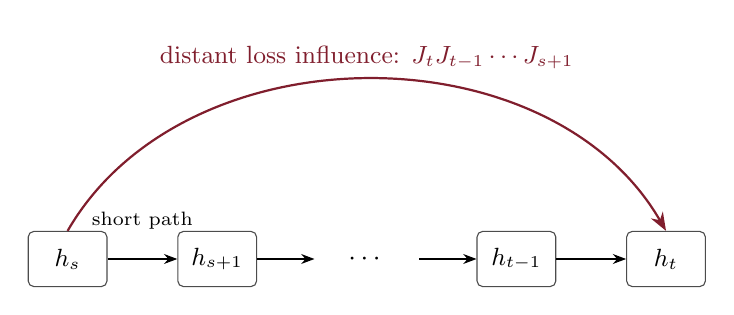
\begin{tikzpicture}[x=1.9cm]
 \foreach \i/\l in {0/{h_s},1/{h_{s+1}},3/{h_{t-1}},4/{h_t}} \node[nbox] (n\i) at (\i,0) {$\l$};
 \node at (2,0) {$\cdots$};
 \draw[->] (n0) -- (n1);
 \draw[->] (n1) -- (1.65,0);
 \draw[->] (2.35,0) -- (n3);
 \draw[->] (n3) -- (n4);
 \node[tick,above] at (0.5,0.25) {short path};
 \draw[->,burg,thick] (n0.north) to[out=60,in=120] node[above,font=\small]{distant loss influence: $J_tJ_{t-1}\cdots J_{s+1}$} (n4.north);
\end{tikzpicture}
\caption{Redrawn from slide 4. The influence of $h_s$ on $h_t$ is a long product of Jacobians; the direct (short) path between neighbouring states is unproblematic.}
\end{figure}

\begin{intuition}
Think of passing a message through a chain of $100$ people who each repeat it slightly quieter (factor $0.9$) --- by the end, $0.9^{100}\approx2.7\cdot10^{-5}$ of the original loudness remains. If each person instead exaggerates ($1.1$ each), the message arrives as $1.1^{100}\approx1.4\cdot10^{4}$ times too loud, and in practice it also gets distorted in direction. The norm bound only \emph{guarantees} vanishing when $\gamma\omega<1$; when it exceeds $1$ the product \emph{can} grow along some directions, it is not forced to. The slide's point: a vanilla RNN has \emph{no dedicated retention mechanism}, so a useful long-lived state is hard to learn even when old information remains predictive.
\end{intuition}

\subsection{What should a recurrent memory do? \sltag{5}}

The slides list three \emph{functional goals} for a learned state update:
\begin{itemize}
 \item \textbf{Remember}: retain a relevant earlier event (A stays A);
 \item \textbf{Forget}: attenuate obsolete information (A becomes weak~A);
 \item \textbf{Update}: incorporate a meaningful new event (A is joined or replaced by B).
\end{itemize}
An irrelevant observation should require little change to the stored information.

\begin{figure}[H]\centering
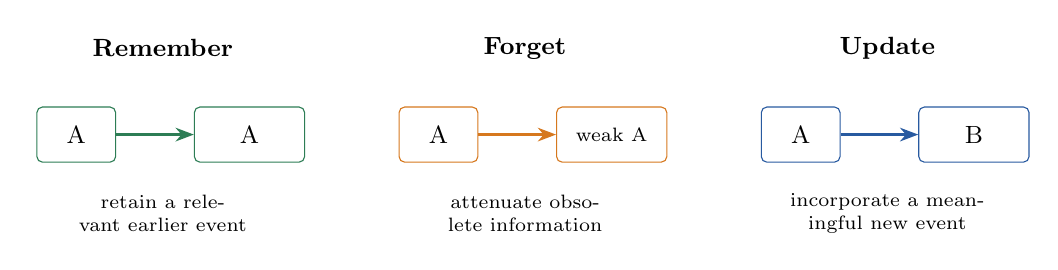
\begin{tikzpicture}
 \foreach \n/\x/\t/\a/\b/\col in {1/0/Remember/A/A/greenc, 2/4.6/Forget/A/{\scriptsize weak A}/orangec, 3/9.2/Update/A/B/bluec}{
  \node[font=\bfseries\small] at (\x+1.1,1.1) {\t};
  \node[nbox,draw=\col] (a\n) at (\x,0) {\a};
  \node[nbox,draw=\col,minimum width=14mm] (b\n) at (\x+2.2,0) {\b};
  \draw[->,\col,thick] (a\n) -- (b\n);
 }
 \node[tick,align=center,text width=3.2cm] at (1.1,-1) {retain a relevant earlier event};
 \node[tick,align=center,text width=3.2cm] at (5.7,-1) {attenuate obsolete information};
 \node[tick,align=center,text width=3.2cm] at (10.3,-1) {incorporate a meaningful new event};
\end{tikzpicture}
\caption{Redrawn from slide 5: the three things a recurrent memory must be able to do.}
\end{figure}

\begin{intuition}
A good memory is an \emph{editable notebook}, not a whiteboard that is wiped and rewritten at each step. Sometimes you keep a line, sometimes you cross it out, sometimes you write a new one --- and on a boring day you write nothing. A vanilla RNN rewrites the whole whiteboard through the same transformation every step; gating gives it a pen, an eraser and the freedom to leave things alone. These are \emph{functional goals}; they say what the update should be able to do, not that every trained network does it.
\end{intuition}

\subsection{A gate is an elementwise soft mask \sltag{6--7}}

\begin{definition}{Gate (soft mask)}{gate}
Let $v_t\in\R^m$ be a vector of signals. A \emph{gate} is a vector $g_t\in(0,1)^m$. The gated signal is the Hadamard product
\[
v_t'=g_t\odot v_t,\qquad v'_{t,j}=g_{t,j}\,v_{t,j}\quad(j=1,\dots,m).
\]
Equivalently $v'_t=\diag(g_t)\,v_t$.
\end{definition}

A coefficient near~$1$ passes a component with little attenuation, a coefficient near~$0$ suppresses it strongly, and intermediate values attenuate it partially. Because $g_t$ is built from sigmoids it is a \emph{continuous} soft mask, in contrast with a hard $0/1$ switch.

\begin{example}{Slide 6}{mask6}
\[
v_t=\vc{2\\-1\\3\\-2},\quad g_t=\vc{0.9\\0.1\\0.5\\0.8}\ \Longrightarrow\ g_t\odot v_t=\vc{1.8\\-0.1\\1.5\\-1.6}.
\]
Components~1 and~4 are mostly passed, component~2 is nearly erased, component~3 is halved. Signs are never flipped, because $g>0$.
\end{example}

\paragraph{Masking in a minibatch (slide 7).} With $B$ examples (rows) and $m$ features (columns) at the same time $t$, the operation is applied entrywise:
\[
V_t\odot G_t=V_t',\qquad V_t,V_t'\in\R^{B\times m},\ G_t\in(0,1)^{B\times m}.
\]
The slide's numbers ($B=3$, $m=4$):
\[
\underbrace{\begin{pmatrix}2&-2&1&2\\-1&1.5&-0.4&2\\1&-2&0.8&2\end{pmatrix}}_{V_t}
\odot
\underbrace{\begin{pmatrix}.95&.90&.25&.50\\.05&.50&.95&.25\\.90&.50&.10&.05\end{pmatrix}}_{G_t}
=
\underbrace{\begin{pmatrix}1.9&-1.8&.25&1\\-.05&.75&-.38&.5\\.9&-1&.08&.1\end{pmatrix}}_{V_t'}
\]
For instance $2\times.95=1.9$ is \emph{retained}, $2\times.50=1$ is \emph{partially} kept and $1\times.05$-type entries such as $-1\times.05=-.05$ are \emph{suppressed}.

\begin{intuition}
A gate is a bank of \emph{dimmer switches}, one per feature (like the sliders of a graphic equaliser). Each row of the minibatch has its \emph{own} slider positions: the mask is not a fixed property of the network but is recomputed for every example and every timestep (see the next subsection). The Hadamard product never mixes features --- feature $j$ only talks to feature $j$ --- so the mask is a cheap, sharp tool for deciding \emph{which coordinates matter now}.
\end{intuition}

\subsection{How gating preserves information from the past \sltag{8}}

An LSTM's cell state $c_{t-1}$ is a learned representation of earlier observations. The part of it that survives to time $t$ is the masked vector
\[
m_t^{\rm old}=f_t\odot c_{t-1}.
\]
\begin{example}{Slide 8}{preserve}
With $c_{t-1}=(2,-2,1,-1)^\top$ and $f_t=(.95,.05,.5,.8)^\top$:
\[
m_t^{\rm old}=(1.9,\,-0.1,\,0.5,\,-0.8)^\top .
\]
In the slide's constructed story, channel~1 stores event~A (kept at $95\%$), channel~2 stores event~B, whose relevance has dropped (kept at only $5\%$).
\end{example}

\begin{intuition}
Retention is simply \emph{multiplication by a number between 0 and 1}: $0.95$ means ``A is still important'', $0.05$ means ``B is almost irrelevant''. The slide warns that the feature meanings here are \emph{predefined for illustration}: in a trained network, state coordinates are learned and rarely correspond to one human-readable event each. Retained content can nevertheless influence later predictions, which is the whole point.
\end{intuition}

\subsection{How are gate values generated? \sltag{9}}

\begin{definition}{Learned gate}{learnedgate}
A learned gate at time $t$ is
\[
g_t=\sigma\big(W_{gx}x_t+W_{gh}h_{t-1}+b_g\big),
\]
where $W_{gx}\in\R^{m\times d}$, $W_{gh}\in\R^{m\times m}$ and $b_g\in\R^m$ are learned, and $\sigma$ acts elementwise.
\end{definition}

\begin{figure}[H]\centering
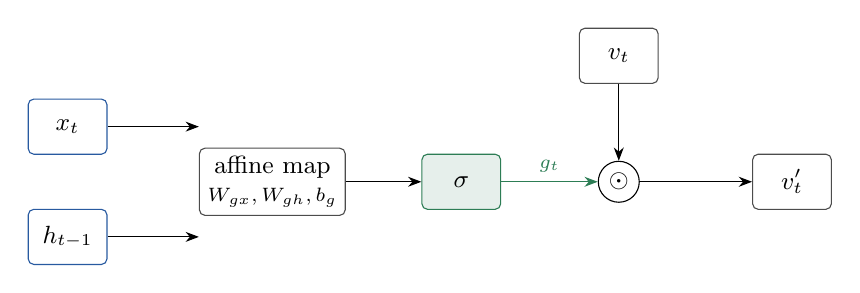
\begin{tikzpicture}
 \node[nbox,draw=bluec] (x) at (0,0.7) {$x_t$};
 \node[nbox,draw=bluec] (h) at (0,-0.7) {$h_{t-1}$};
 \node[nbox,align=center] (aff) at (2.6,0) {affine map\\[-1pt]\scriptsize $W_{gx},W_{gh},b_g$};
 \node[gbox] (sg) at (5.0,0) {$\sigma$};
 \node[mul] (mu) at (7.0,0) {$\odot$};
 \node[nbox] (v) at (7.0,1.6) {$v_t$};
 \node[nbox] (vp) at (9.2,0) {$v_t'$};
 \draw[->] (x) -- (aff.west |- x);\draw[->] (h) -- (aff.west |- h);
 \draw[->] (aff) -- (sg);
 \draw[->,greenc] (sg) -- node[above,tick]{$g_t$} (mu);
 \draw[->] (v) -- (mu);
 \draw[->] (mu) -- (vp);
\end{tikzpicture}
\caption{Redrawn from slide 9: a gate is an affine function of the current input and previous hidden state, squashed by a sigmoid, then multiplied onto a signal $v_t$.}
\end{figure}

$W_{gx}x_t$ supplies current-input features and $W_{gh}h_{t-1}$ supplies temporal context. The matrices and bias are \emph{parameters} (shared across time); the gate \emph{values} are \emph{activations}, computed anew for every timestep and every example.

\begin{intuition}
A gate is a tiny learned decision-maker: ``given what I see now and what I remember, how open should each channel be?'' Because it reads $x_t$ and $h_{t-1}$, the network can decide to hold on to information when the input is uninteresting and to let go when a relevant new event arrives. The \emph{parameters} fix the decision rule; the \emph{values} are its decisions.
\end{intuition}

\subsection{The sigmoid supplies continuous control \sltag{10}}

\begin{proposition}{Properties of the logistic sigmoid}{sigmoid}
For $\sigma(a)=1/(1+e^{-a})$:
\begin{enumerate}[label=(\roman*)]
 \item $\sigma(a)\in(0,1)$ for every finite $a$, $\sigma$ is strictly increasing and $\sigma(-a)=1-\sigma(a)$;
 \item $\sigma'(a)=\sigma(a)\big(1-\sigma(a)\big)\in(0,\tfrac14]$, with maximum $\tfrac14$ at $a=0$;
 \item $\sigma'(a)\le e^{-|a|}$ (saturation).
\end{enumerate}
\end{proposition}
\begin{proof}
(i) is immediate from the formula. (ii) Differentiating, $\sigma'(a)=e^{-a}/(1+e^{-a})^2$, and since $1-\sigma(a)=e^{-a}/(1+e^{-a})$ this equals $\sigma(a)(1-\sigma(a))$, a concave parabola in $\sigma$ maximised at $\sigma=\tfrac12$. (iii) $\sigma'(a)=1/(e^{a/2}+e^{-a/2})^2=1/(4\cosh^2(a/2))$ and $\cosh(u)\ge e^{|u|}/2$, hence $4\cosh^2(a/2)\ge e^{|a|}$.
\end{proof}

\begin{figure}[H]\centering
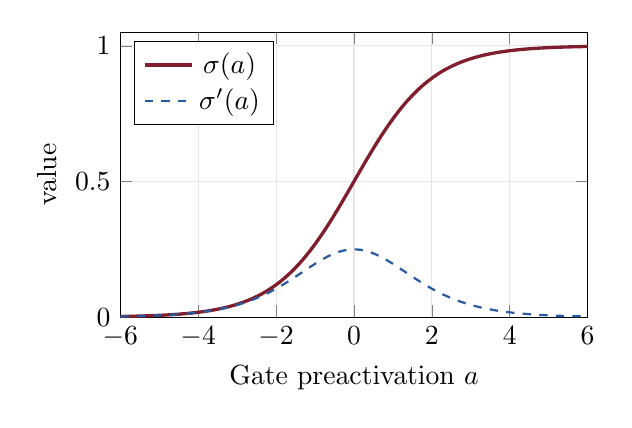
\begin{tikzpicture}
\begin{axis}[width=0.62\linewidth,height=5.2cm,xlabel={Gate preactivation $a$},ylabel={value},xmin=-6,xmax=6,ymin=0,ymax=1.05,
 legend pos=north west,grid=both,grid style={gray!20}]
 \addplot[burg,very thick,domain=-6:6,samples=100]{1/(1+exp(-x))};
 \addlegendentry{$\sigma(a)$}
 \addplot[bluec,thick,dashed,domain=-6:6,samples=100]{(1/(1+exp(-x)))*(1-1/(1+exp(-x)))};
 \addlegendentry{$\sigma'(a)$}
\end{axis}
\end{tikzpicture}
\caption{Sigmoid gate (slide 10) together with its derivative (added here): the gate is soft and strictly between $0$ and $1$, but its derivative vanishes in the saturated regions.}
\end{figure}

\begin{intuition}
The sigmoid is a smooth dimmer: it maps any real preactivation to a coefficient in $(0,1)$, so the gate can be \emph{trained by gradient descent} (a hard $0/1$ switch has zero gradient almost everywhere). The price is saturation: at $a=\pm6$ the slope is only $\approx0.0025$, so a gate that is firmly open or shut learns slowly. The slide's warning --- ``gate learning still depends on optimization'' --- is exactly this.
\end{intuition}

\begin{remarkbox}[Supplementary: initial gate bias]
Since $\sigma(b)$ is the gate value when the weights contribute nothing, the bias sets the initial ``default'' behaviour: $\sigma(3)\approx0.95$ makes a forget gate retain by default. This is a common practical choice, not something derived on the slides.
\end{remarkbox}

\subsection{Selective retention through gated interpolation \sltag{11}}

One illustrative update mixes the previous state and a candidate:
\[
s_t=g_t\odot s_{t-1}+(1-g_t)\odot\tilde s_t .
\]
\begin{example}{Slide 11}{interp}
$s_{t-1}=(4,-2)^\top$, $\tilde s_t=(0,3)^\top$, $g_t=(0.8,0.2)^\top$. The retained part is $g_t\odot s_{t-1}=(3.2,-0.4)^\top$; the written part is $(1-g_t)\odot\tilde s_t=(0.2,0.8)^\top\odot(0,3)^\top=(0,2.4)^\top$. Therefore $s_t=(3.2,\,2.0)^\top$.
\end{example}

\begin{proposition}{Gated interpolation is a convex combination}{convex}
For each coordinate $j$, $s_{t,j}$ lies between $s_{t-1,j}$ and $\tilde s_{t,j}$. Consequently, if $|s_{0,j}|\le1$ and $|\tilde s_{t,j}|\le1$ for all $t$, then $|s_{t,j}|\le1$ for all $t$.
\end{proposition}
\begin{proof}
$s_{t,j}=g\,s_{t-1,j}+(1-g)\tilde s_{t,j}$ with $g\in(0,1)$ is a weighted average with positive weights summing to one, hence lies between the two values. If $|s_{t-1,j}|\le1$ and $|\tilde s_{t,j}|\le1$ then the average has modulus at most $1$; induct on $t$.
\end{proof}

\begin{intuition}
Each coordinate has its own \emph{cross-fader} between ``keep what I had'' and ``take the new proposal''. At $g=0.8$ the old value dominates, at $g=0.2$ the new one does (the two coordinates of the example behave in exactly opposite ways). Because the result is an average, the state cannot blow up if the candidate is bounded --- a useful stability property. The slide stresses this is a \emph{generic} interpolation; real architectures can combine gates differently (the LSTM, for example, does not tie the write weight to $1-f_t$).
\end{intuition}

\subsection{Why additive memory pathways matter \sltag{12}}

\begin{figure}[H]\centering
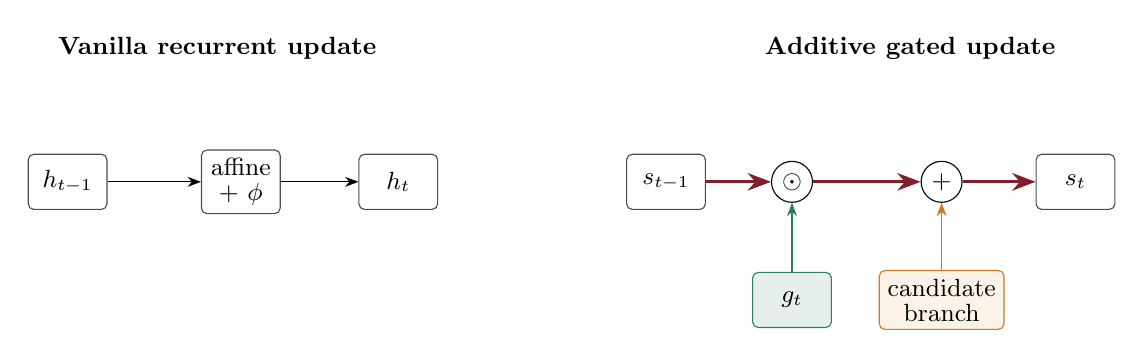
\begin{tikzpicture}
 \node[font=\bfseries\small] at (1.9,1.7) {Vanilla recurrent update};
 \node[nbox] (a) at (0,0) {$h_{t-1}$};
 \node[nbox,align=center] (b) at (2.2,0) {affine\\[-2pt]$+\ \phi$};
 \node[nbox] (c) at (4.2,0) {$h_t$};
 \draw[->] (a)--(b); \draw[->] (b)--(c);
 \node[font=\bfseries\small] at (10.7,1.7) {Additive gated update};
 \node[nbox] (s0) at (7.6,0) {$s_{t-1}$};
 \node[mul] (m) at (9.2,0) {$\odot$};
 \node[mul] (p) at (11.1,0) {$+$};
 \node[nbox] (s1) at (12.8,0) {$s_t$};
 \node[nbox,draw=orangec,align=center,fill=orangec!10] (cand) at (11.1,-1.5) {candidate\\[-2pt]branch};
 \node[gbox] (gt) at (9.2,-1.5) {$g_t$};
 \draw[->,cellp] (s0)--(m); \draw[->,cellp] (m)--(p); \draw[->,cellp] (p)--(s1);
 \draw[->,greenc] (gt)--(m); \draw[->,orangec] (cand)--(p);
\end{tikzpicture}
\caption{Redrawn from slide 12. Left: every step applies the recurrent transformation and activation. Right: the memory travels along a direct elementwise path.}
\end{figure}

\begin{proposition}{Direct path of a gated additive update}{directpath}
Let $s_t=g_t\odot s_{t-1}+u_t$ and hold $g_t,u_t$ fixed. Then $\partial s_t/\partial s_{t-1}\big|_{\rm direct}=\diag(g_t)$, and over $k=t-s$ steps
\[
\left.\frac{\partial s_t}{\partial s_s}\right|_{\rm direct}=\diag(g_t\odot\cdots\odot g_{s+1}).
\]
Moreover, for any $s<t$ the state unrolls as
\[
s_t=\underbrace{\Big(\textstyle\bigodot_{j=s+1}^{t}g_j\Big)}_{P_{s:t}}\odot s_s+\sum_{k=s+1}^{t}\Big(\textstyle\bigodot_{j=k+1}^{t}g_j\Big)\odot u_k ,
\]
with the empty Hadamard product equal to the all-ones vector.
\end{proposition}
\begin{proof}
The first statement is differentiation of $g_t\odot s_{t-1}$ with $g_t$ fixed. For the unrolled form: for $t=s+1$ it reads $s_{s+1}=g_{s+1}\odot s_s+u_{s+1}$. Assume it holds at $t$; then
$s_{t+1}=g_{t+1}\odot s_t+u_{t+1}=P_{s:t+1}\odot s_s+\sum_{k=s+1}^{t}\big(\bigodot_{j=k+1}^{t+1}g_j\big)\odot u_k+u_{t+1}$, which is the formula at $t+1$ (the last term is the $k=t+1$ summand with an empty product).
\end{proof}

\begin{intuition}
In a vanilla RNN every step pushes the memory through $W_h$ and a nonlinearity --- like photocopying a photocopy, each generation a bit more distorted. In the additive form the memory rides a \emph{conveyor belt}: it is only scaled by the gate and then new content is \emph{added}. If the gate stays near $1$ the memory survives almost untouched: with $g=0.99$ and $100$ steps, $0.99^{100}\approx0.37$ survives, against $0.9^{100}\approx2.7\cdot10^{-5}$ for a contracting factor $0.9$. The unrolled formula shows that old content is a \emph{weighted sum} of past writes, each attenuated by the product of the later gates. The slide's caveat: the full Jacobian also contains gate and candidate dependencies, so additive pathways \emph{support} retention only when the gate dynamics are favourable.
\end{intuition}

\subsection{From soft masks to an LSTM \sltag{13}}

An LSTM combines a persistent \emph{cell-state pathway} with learned control signals. It has two recurrent quantities: the \textbf{cell state} $c_t$, which stores evolving information, and a separately controlled \textbf{hidden state} $h_t$, which feeds the readout and subsequent recurrent computations. Learned \textbf{gates} and a \textbf{candidate memory} decide what is erased and what is written. The next section builds each operation separately before assembling the complete cell.

\begin{intuition}
The LSTM is the soft-mask idea above, made concrete: a \emph{notebook} ($c_t$) that is edited with eraser and pen under the control of gates, and a \emph{spokesperson} ($h_t$) who reports a filtered view of the notebook to the rest of the network.
\end{intuition}
%=====================================================================
\section{Long Short-Term Memory Networks (LSTMs) \sltag{14--33}}
%=====================================================================

\subsection{Why introduce an LSTM? \sltag{14}}

Hochreiter and Schmidhuber introduced Long Short-Term Memory in 1997 to support learning over extended temporal intervals \cite{r5}. The now-standard \emph{forget gate} was added later, in work on continual prediction by Gers, Schmidhuber and Cummins (2000) \cite{r6}.

\begin{figure}[H]\centering
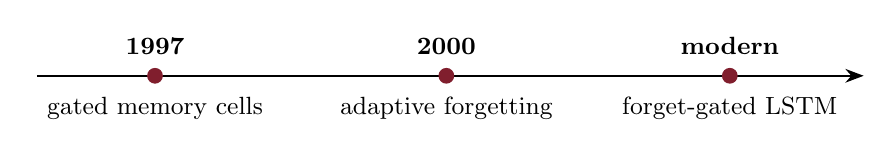
\begin{tikzpicture}
 \draw[thick,->] (0,0) -- (10.5,0);
 \foreach \x/\y/\t in {1.5/1997/{gated memory cells},5.2/2000/{adaptive forgetting},8.8/modern/{forget-gated LSTM}}{
  \fill[burg] (\x,0) circle (0.1);
  \node[above,font=\bfseries\small] at (\x,0.15) {\y};
  \node[below,font=\small,text width=3cm,align=center] at (\x,-0.15) {\t};
 }
\end{tikzpicture}
\caption{Redrawn from slide 14: milestones of the LSTM.}
\end{figure}

These notes develop the standard \emph{no-peephole, no-projection} variant used in the lecture. Its pathways help address long-term learning difficulties, but their usefulness still depends on the data, the gate dynamics and optimisation \cite{r7}.

\subsection{Two recurrent quantities carry different information \sltag{15}}

\begin{definition}{LSTM state}{lstmstate}
An LSTM carries the pair $(h_t,c_t)$, both in $\R^m$: the \emph{cell state} $c_t$ is the explicit cell-memory pathway; the \emph{hidden state} $h_t$ is the exposed representation used by recurrent computations and by the readout. Both are initialised at sequence boundaries, e.g.\ $h_0=c_0=0$.
\end{definition}

\begin{figure}[H]\centering
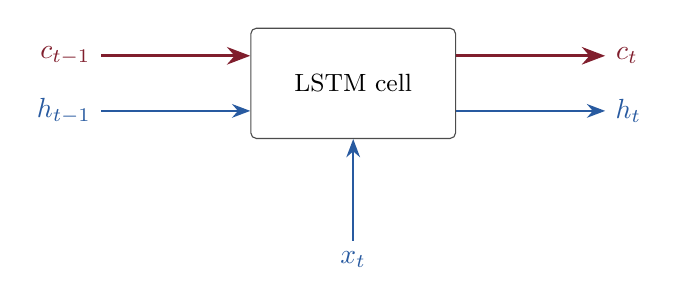
\begin{tikzpicture}
 \node[nbox,minimum width=26mm,minimum height=14mm] (cell) at (0,0) {LSTM cell};
 \draw[->,cellp] (-3.2,0.35) node[left]{$c_{t-1}$} -- (cell.west |- 0,0.35);
 \draw[->,cellp] (cell.east |- 0,0.35) -- (3.2,0.35) node[right]{$c_t$};
 \draw[->,busp] (-3.2,-0.35) node[left]{$h_{t-1}$} -- (cell.west |- 0,-0.35);
 \draw[->,busp] (cell.east |- 0,-0.35) -- (3.2,-0.35) node[right]{$h_t$};
 \draw[->,busp] (0,-2) node[below]{$x_t$} -- (cell.south);
\end{tikzpicture}
\caption{Redrawn from slide 15: two recurrent channels enter and leave each LSTM cell.}
\end{figure}

\begin{intuition}
Why two vectors? $c_t$ is the \emph{private notebook}, edited by erase-and-add; $h_t$ is what the cell \emph{chooses to show} to the readout and to the next step's gates. Separating them lets the network keep something in memory without constantly broadcasting it.
\end{intuition}

\subsection{Each gate has its own learned parameters \sltag{16}}

\begin{definition}{LSTM gates}{lstmgates}
For $k\in\{f,i,o\}$ (forget, input, output),
\[
g_t^{(k)}=\sigma\big(W_{kx}x_t+W_{kh}h_{t-1}+b_k\big),\qquad W_{kx}\in\R^{m\times d},\ W_{kh}\in\R^{m\times m},\ b_k\in\R^m .
\]
In the standard variant used here the gate preactivations have no direct cell-state input (no peepholes).
\end{definition}

The three gates use separate parameter sets but read the \emph{same} current input and previous hidden state; each produces its own componentwise coefficients in $(0,1)^m$. We write $f_t,i_t,o_t$ for $g_t^{(f)},g_t^{(i)},g_t^{(o)}$.

\subsection{The forget gate selects previous cell content \sltag{17}}

\[
f_t=\sigma(W_{fx}x_t+W_{fh}h_{t-1}+b_f),\qquad m_t^{\rm old}=f_t\odot c_{t-1}.
\]
The forget gate controls retention on the direct cell-state pathway \cite{r6}.

\begin{example}{Slide 17}{forget}
$c_{t-1}=(2,-1,3)^\top$, $f_t=(.9,.1,.5)^\top$ give $m_t^{\rm old}=(1.8,-0.1,1.5)^\top$: feature~1 keeps $90\%$ of its value, feature~2 keeps $10\%$, feature~3 keeps half; the sign of each activation is preserved.
\end{example}

\begin{intuition}
The forget gate is the \emph{eraser}: $f=1$ means ``leave this note untouched'', $f=0$ means ``wipe it''. The name is slightly backwards --- a high forget-gate value means \emph{remember}.
\end{intuition}

\subsection{Candidate memory proposes new content \sltag{18}}

\[
\tc_t=\tanh(W_{cx}x_t+W_{ch}h_{t-1}+b_c)\in(-1,1)^m .
\]
The candidate proposes \emph{signed} content; it determines \emph{what could be written} into memory, while the input gate separately controls \emph{how much} is written.

\begin{figure}[H]\centering
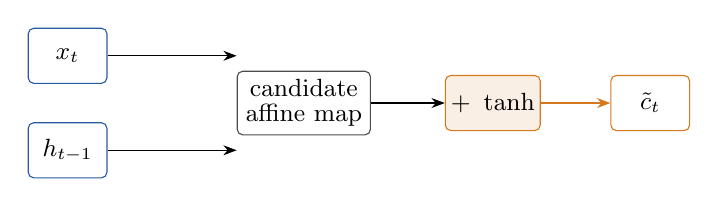
\begin{tikzpicture}
 \node[nbox,draw=bluec] (x) at (0,0.6) {$x_t$};
 \node[nbox,draw=bluec] (h) at (0,-0.6) {$h_{t-1}$};
 \node[nbox,align=center] (aff) at (3,0) {candidate\\[-2pt]affine map};
 \node[cbox] (t) at (5.4,0) {$+\ \tanh$};
 \node[nbox,draw=orangec] (c) at (7.4,0) {$\tc_t$};
 \draw[->] (x)--(aff.west|-x); \draw[->] (h)--(aff.west|-h); \draw[->](aff)--(t);\draw[->,orangec](t)--(c);
\end{tikzpicture}
\caption{Redrawn from slide 18: generation of the candidate memory.}
\end{figure}

\subsection{The input gate selects what to write \sltag{19}}

\[
i_t=\sigma(W_{ix}x_t+W_{ih}h_{t-1}+b_i),\qquad m_t^{\rm new}=i_t\odot\tc_t .
\]
\begin{example}{Slide 19}{inputgate}
$\tc_t=(.5,-.8,.2)^\top$, $i_t=(.2,.9,.5)^\top$ give $m_t^{\rm new}=(.1,-.72,.1)^\top$. The second feature is written strongly, with its negative sign; the first is attenuated to one fifth of its proposed value.
\end{example}

\begin{intuition}
The input gate is the \emph{pen pressure}: the candidate is what you would like to write, the input gate says how hard to press. Splitting ``what'' (candidate) from ``how much'' (gate) lets the network propose something and then decline to commit to it.
\end{intuition}

\subsection{The central cell-state update \sltag{20--21}}

\begin{definition}{LSTM cell-state update}{cellupdate}
\[
c_t=\underbrace{f_t\odot c_{t-1}}_{m_t^{\rm old}}+\underbrace{i_t\odot\tc_t}_{m_t^{\rm new}} .
\]
\end{definition}

\begin{example}{Slide 20}{update}
\[
\underbrace{(2,-1,3)^\top\odot(.9,.1,.5)^\top}_{=(1.8,\,-.1,\,1.5)^\top}+\underbrace{(.5,-.8,.2)^\top\odot(.2,.9,.5)^\top}_{=(.1,\,-.72,\,.1)^\top}=(1.9,\,-0.82,\,1.6)^\top .
\]
Here $f_t+i_t=(1.1,1,1)^\top$: the two gates are independent, so the sums need not equal one --- both can even be large or small at the same time.
\end{example}

\paragraph{One component at a time (slide 21).} For a single coordinate, $c_t=f_tc_{t-1}+i_t\tc_t$:
\begin{center}
\begin{tabular}{lccccc}\toprule
Operation & $c_{t-1}$ & $f_t$ & $i_t$ & $\tc_t$ & $c_t$\\ \midrule
Mostly retain & 2 & 0.99 & 0.01 & 0.5 & 1.985\\
Mostly replace & 2 & 0.05 & 0.90 & $-0.5$ & $-0.35$\\
Retain and add & 2 & 0.90 & 0.80 & 0.5 & 2.20\\ \bottomrule
\end{tabular}
\end{center}
(These coefficients are hand-chosen to explain the algebra.) Check: $2(.99)+.01(.5)=1.985$; $2(.05)+.9(-.5)=-.35$; $2(.9)+.8(.5)=2.2$.

\begin{proposition}{Unrolling the cell state; size of the cell}{cellunroll}
Applying Proposition~\ref{prop:directpath} with $g_t=f_t$ and $u_t=i_t\odot\tc_t$,
\[
c_t=\Big(\textstyle\bigodot_{j=s+1}^{t}f_j\Big)\odot c_s+\sum_{k=s+1}^{t}\Big(\textstyle\bigodot_{j=k+1}^{t}f_j\Big)\odot i_k\odot\tc_k .
\]
Moreover $|c_{t,j}|<|c_{t-1,j}|+1$, hence $|c_{t,j}|\le|c_{0,j}|+t$; and if $f_{t,j}+i_{t,j}\le1$ at all steps then $|c_{t,j}|\le\max(|c_{0,j}|,1)$. In particular the cell state can exceed $[-1,1]$ although the candidate uses $\tanh$.
\end{proposition}
\begin{proof}
The unrolled identity is the general formula. For the bounds: $|c_{t,j}|\le f|c_{t-1,j}|+i|\tc_{t,j}|<|c_{t-1,j}|+1$ since $f,i\in(0,1)$, $|\tc|<1$. If $f+i\le1$, then $|c_{t,j}|\le (f+i)\max(|c_{t-1,j}|,1)\le\max(|c_{t-1,j}|,1)$; induct.
\end{proof}

\begin{intuition}
Read the table rows as three behaviours: \emph{hold the old note} ($f\approx1,i\approx0$), \emph{overwrite it} ($f\approx0,i$ large), and \emph{keep it and add more} ($f$ and $i$ both large) --- the last one is why the cell can accumulate beyond the candidate's range of $(-1,1)$. Independent retention and writing is what an LSTM adds over the tied interpolation of the previous section.
\end{intuition}

\subsection{The output gate controls exposed memory \sltag{22}}

\[
o_t=\sigma(W_{ox}x_t+W_{oh}h_{t-1}+b_o),\qquad h_t=o_t\odot\tanh(c_t).
\]
The output gate regulates which cell features are exposed. A small output gate suppresses the exposed representation while the stored cell content continues along its own temporal pathway.

\begin{proposition}{Hidden state is bounded}{hbound}
$h_{t,j}\in(-1,1)$ for all $t,j$.
\end{proposition}
\begin{proof}
$o_{t,j}\in(0,1)$ and $\tanh(c_{t,j})\in(-1,1)$.
\end{proof}

\begin{intuition}
Closing the output gate means ``don't show this to the rest of the network right now'' --- it does \emph{not} delete the memory. The cell can keep a fact hidden for hundreds of steps and reveal it only when it becomes relevant. The $\tanh$ compresses the (possibly large) cell value into a bounded range before it is exposed.
\end{intuition}

\subsection{Hidden state and prediction are separate outputs \sltag{23}}

The exposed hidden state can feed a task-specific readout
\[
a_t^{y}=W_yh_t+b_y,\qquad\hat y_t=\psi(a_t^{y}),\qquad W_y\in\R^{q\times m},\ b_y\in\R^q,\ \hat y_t\in\R^q .
\]
Regression may use $\psi=\mathrm{id}$; classification can use softmax. Notation warning from the slide: $o_t$ is the LSTM \emph{output gate}; the \emph{prediction} is $\hat y_t$. The next recurrent step receives both $h_t$ and $c_t$.

\subsection{Assembling the cell: the information pathways \sltag{24--29}}

The slides build the cell in four stages; Figure~\ref{fig:lstmbuild} reproduces them (burgundy: cell memory, orange: candidate content, green: gate masks, blue: input and hidden-state features).

\newcommand{\lstmfig}[1]{%
\begin{tikzpicture}[scale=1]
 \useasboundingbox (-3.4,-0.3) rectangle (11.6,4.4);
 \def\stg{#1}
 \pgfmathtruncatemacro{\stgn}{\stg}
 \edef\busend{\ifcase\stgn\or 2\or 5.5\or 5.5\or 7\fi}
 % bus
 \draw[busp] (-1.0,0.3) -- (\busend,0.3);
 \node[left,font=\small] at (-1.0,0.3) {$[x_t;h_{t-1}]$};
 % stage 1 : retention
 \node[left,font=\small] at (-0.9,4) {$c_{t-1}$};
 \node[mul] (mf) at (2,4) {$\odot$};
 \node[gbox] (sf) at (2,1.4) {$\sigma_f$};
 \draw[->,busp] (2,0.3) -- (sf.south);
 \draw[->,greenc] (sf.north) -- node[right,tick]{$f_t$} (mf.south);
 \draw[cellp] (-0.9,4) -- (mf.west);
 \ifnum\stgn<3
  \draw[->,cellp] (mf.east) -- node[above,tick]{$m^{\rm old}_t$} (3.6,4);
 \fi
 % stage 2 : candidate write
 \ifnum\stgn>1
  \node[gbox] (si) at (3.7,1.4) {$\sigma_i$};
  \node[cbox] (tc) at (5.5,1.4) {$\tanh_c$};
  \node[mul] (mi) at (4.6,2.7) {$\odot$};
  \draw[->,busp] (3.7,0.3) -- (si.south);
  \draw[->,busp] (5.5,0.3) -- (tc.south);
  \draw[->,greenc] (si.north) -- node[left,tick]{$i_t$} (3.7,2.7) -- (mi.west);
  \draw[->,orangec] (tc.north) -- node[right,tick]{$\tilde c_t$} (5.5,2.7) -- (mi.east);
 \fi
 \ifnum\stgn=2
  \draw[->,cellp] (mi.north) -- node[left,tick]{$m^{\rm new}_t$} (4.6,3.7);
 \fi
 % stage 3 : addition
 \ifnum\stgn>2
  \node[mul] (pl) at (4.6,4) {$+$};
  \draw[cellp] (mf.east) -- node[above,tick]{$m^{\rm old}_t$} (pl.west);
  \draw[->,cellp] (mi.north) -- node[left,tick]{$m^{\rm new}_t$} (pl.south);
  \ifnum\stgn=3
   \draw[->,cellp] (pl.east) -- (10.4,4) node[right]{$c_t$};
  \else
   \draw[cellp] (pl.east) -- (10.4,4);
   \node[right] at (10.4,4) {$c_t$};
  \fi
 \fi
 % stage 4 : output
 \ifnum\stgn>3
  \node[gbox] (so) at (7,1.4) {$\sigma_o$};
  \node[mul] (mo) at (8.4,2.2) {$\odot$};
  \node[tbox] (th) at (8.4,3.1) {$\tanh$};
  \draw[->,busp] (7,0.3) -- (so.south);
  \draw[->,greenc] (so.north) -- node[right,tick]{$o_t$} (7,2.2) -- (mo.west);
  \draw[->,cellp] (8.4,4) -- (th.north);
  \fill[burg] (8.4,4) circle (0.06);
  \draw[->,cellp] (th.south) -- (mo.north);
  \draw[->,busp] (mo.east) -- (10.4,2.2) node[right]{$h_t$};
 \fi
\end{tikzpicture}}

\begin{figure}[H]\centering
\begin{minipage}{0.49\linewidth}\centering\resizebox{\linewidth}{!}{\lstmfig{1}}\\[-1pt]{\small (a) retention path (slide 24)}\end{minipage}\hfill
\begin{minipage}{0.49\linewidth}\centering\resizebox{\linewidth}{!}{\lstmfig{2}}\\[-1pt]{\small (b) candidate write path (slide 25)}\end{minipage}\\[6pt]
\begin{minipage}{0.49\linewidth}\centering\resizebox{\linewidth}{!}{\lstmfig{3}}\\[-1pt]{\small (c) adding the two contributions (slide 26)}\end{minipage}\hfill
\begin{minipage}{0.49\linewidth}\centering\resizebox{\linewidth}{!}{\lstmfig{4}}\\[-1pt]{\small (d) exposing the hidden state (slide 27)}\end{minipage}
\caption{Progressive construction of the LSTM cell, redrawn from slides 24--27. (a) $m_t^{\rm old}=f_t\odot c_{t-1}$. (b) $m_t^{\rm new}=i_t\odot\tc_t$. (c) $c_t=m_t^{\rm old}+m_t^{\rm new}$. (d) $h_t=o_t\odot\tanh(c_t)$.}
\label{fig:lstmbuild}
\end{figure}

\begin{figure}[H]\centering
\lstmfig{4}
\caption{The complete LSTM cell (slide 28). Each $\sigma_k$ box includes its own affine map of $[x_t;h_{t-1}]$; the $\tanh_c$ box includes the candidate affine map. The output gate acts on the transformed \emph{new} cell state.}
\label{fig:lstmfull}
\end{figure}

\begin{algorithm}{LSTM forward step (slide 29)}{lstmstep}
Given $x_t$, $h_{t-1}$, $c_{t-1}$:
\begin{align*}
f_t&=\sigma(W_{fx}x_t+W_{fh}h_{t-1}+b_f), & i_t&=\sigma(W_{ix}x_t+W_{ih}h_{t-1}+b_i),\\
o_t&=\sigma(W_{ox}x_t+W_{oh}h_{t-1}+b_o), & \tc_t&=\tanh(W_{cx}x_t+W_{ch}h_{t-1}+b_c),\\
c_t&=f_t\odot c_{t-1}+i_t\odot\tc_t, & h_t&=o_t\odot\tanh(c_t).
\end{align*}
The gate and candidate maps can be evaluated together from the same incoming data (one large matrix multiplication). The same parameter sets are used at every timestep.
\end{algorithm}

\begin{intuition}
Follow the burgundy line: the cell state enters on the left, passes the \emph{eraser} ($\odot f$), receives the \emph{new writing} ($+\,i\odot\tilde c$) and leaves on the right --- the only operations on it are an elementwise multiplication and an addition, no matrix multiplication. Everything else (green and orange boxes) is a controller that looks at $[x_t;h_{t-1}]$ and sets the dials. Finally the output gate decides how much of $\tanh(c_t)$ is shown as $h_t$.
\end{intuition}

\subsection{Unfolding an LSTM keeps both recurrent channels \sltag{30}}

\begin{figure}[H]\centering
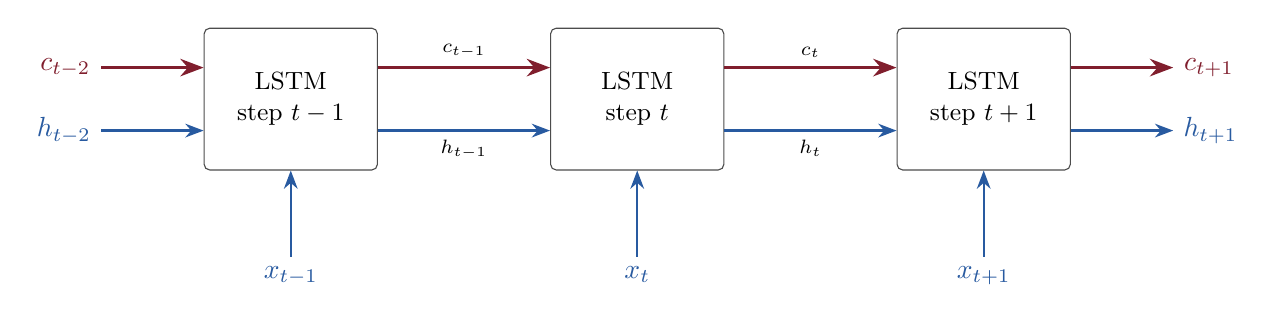
\begin{tikzpicture}
 \foreach \k/\l/\xx in {0/{t-1}/0, 1/{t}/4.4, 2/{t+1}/8.8}{
  \node[nbox,minimum width=22mm,minimum height=18mm,align=center] (b\k) at (\xx,0) {LSTM\\step $\l$};
  \draw[->,busp] (\xx,-2) node[below]{$x_{\l}$} -- (b\k.south);
 }
 \foreach \k/\n in {0/1,1/2}{
  \draw[->,cellp] ($(b\k.east)+(0,0.4)$) -- ($(b\n.west)+(0,0.4)$);
  \draw[->,busp] ($(b\k.east)+(0,-0.4)$) -- ($(b\n.west)+(0,-0.4)$);
 }
 \draw[->,cellp] ($(b0.west)+(-1.3,0.4)$) node[left]{$c_{t-2}$} -- ($(b0.west)+(0,0.4)$);
 \draw[->,busp] ($(b0.west)+(-1.3,-0.4)$) node[left]{$h_{t-2}$} -- ($(b0.west)+(0,-0.4)$);
 \draw[->,cellp] ($(b2.east)+(0,0.4)$) -- ($(b2.east)+(1.3,0.4)$) node[right]{$c_{t+1}$};
 \draw[->,busp] ($(b2.east)+(0,-0.4)$) -- ($(b2.east)+(1.3,-0.4)$) node[right]{$h_{t+1}$};
 \node[tick,above] at ($(b0.east)!0.5!(b1.west)+(0,0.4)$) {$c_{t-1}$};
 \node[tick,below] at ($(b0.east)!0.5!(b1.west)+(0,-0.4)$) {$h_{t-1}$};
 \node[tick,above] at ($(b1.east)!0.5!(b2.west)+(0,0.4)$) {$c_{t}$};
 \node[tick,below] at ($(b1.east)!0.5!(b2.west)+(0,-0.4)$) {$h_{t}$};
\end{tikzpicture}
\caption{Redrawn from slide 30: every cell receives its current input and \emph{both} incoming recurrent quantities; all cells reuse the same gate and candidate parameters.}
\end{figure}

\begin{intuition}
Unfolding in time is just copy-pasting the cell along the sequence with shared weights. The new feature compared with a vanilla RNN is that two lanes run in parallel: a ``slow lane'' $c$ (burgundy) that only gets scaled and added to, and a ``fast lane'' $h$ (blue) that is recomputed from $c$ and re-enters every gate.
\end{intuition}

% \subsection{The direct cell-state edge carries a simple derivative \sltag{31}}

% For the direct memory edge, holding the other incoming node $h_{t-1}$ fixed,
% \[
% \left.\frac{\partial c_t}{\partial c_{t-1}}\right|_{\rm direct}=\diag(f_t).
% \]
% \begin{figure}[H]\centering
% \begin{tikzpicture}
%  \foreach \i/\x in {1/0,2/3.2,3/6.4}{
%   \node[nbox,draw=burg] (c\i) at (\x,1.3) {$c_\i$};
%   \node[nbox,draw=bluec] (h\i) at (\x,0) {$h_\i$};
%  }
%  \draw[->,cellp] (c1)--node[above,tick]{$\diag(f_2)$}(c2);
%  \draw[->,cellp] (c2)--node[above,tick]{$\diag(f_3)$}(c3);
%  \draw[->,busp] (h1)--(h2); \draw[->,busp](h2)--(h3);
%  \draw[->,dashed,gray] (c1)--(h2); \draw[->,dashed,gray](c2)--(h3);
%  \draw[->,dashed,gray] (h1)--(c2); \draw[->,dashed,gray](h2)--(c3);
%  \node[tick,align=left,anchor=west] at (7.4,1.3) {direct memory edge:\\ $\diag(f_t)$};
%  \node[tick,align=left,anchor=west] at (7.4,0) {vanilla RNN edge:\\ $\diag(\phi')W_h$};
% \end{tikzpicture}
% \caption{Adapted from slide 31. Solid burgundy: direct cell-state edges. Dashed grey: the additional routes (through hidden states, gates and candidate) that the full Jacobian also contains.}
% \end{figure}

% \begin{proposition}{Full LSTM Jacobian of $c_t$ with respect to $c_{t-1}$ (supplementary)}{lstmjac}
% Treat $x_t$, $h_{t-2}$ as fixed. With $h_{t-1}=o_{t-1}\odot\tanh(c_{t-1})$ and $D_{t-1}=\diag\big(o_{t-1}\odot(1-\tanh^2(c_{t-1}))\big)$,
% \[
% \begin{aligned}
% \frac{\partial c_t}{\partial c_{t-1}}={}&\diag(f_t)+\Big[\diag\big(c_{t-1}\odot f_t\odot(1-f_t)\big)W_{fh}+\diag\big(\tc_t\odot i_t\odot(1-i_t)\big)W_{ih}\\
% &\qquad+\diag\big(i_t\odot(1-\tc_t^{\,2})\big)W_{ch}\Big]D_{t-1}.
% \end{aligned}
% \]
% \end{proposition}
% \begin{proof}
% $c_t=f_t\odot c_{t-1}+i_t\odot\tc_t$, and $f_t,i_t,\tc_t$ depend on $c_{t-1}$ only through $h_{t-1}$ ($o_{t-1}$ depends on $x_{t-1},h_{t-2}$, not on $c_{t-1}$). The first term gives $\diag(f_t)$. Differentiating the others with $\sigma'=\sigma(1-\sigma)$, $\tanh'=1-\tanh^2$: $\partial(f_t\odot c_{t-1})/\partial h_{t-1}=\diag(c_{t-1}\odot f_t\odot(1-f_t))W_{fh}$, $\partial(i_t\odot\tc_t)/\partial h_{t-1}=\diag(\tc_t\odot i_t(1-i_t))W_{ih}+\diag(i_t\odot(1-\tc_t^2))W_{ch}$, and $\partial h_{t-1}/\partial c_{t-1}=D_{t-1}$.
% \end{proof}

% \begin{intuition}
% In a vanilla RNN \emph{every} path from $h_{t-1}$ to $h_t$ goes through $W_h$. In the LSTM there is an extra ``express lane'' whose derivative is simply $\diag(f_t)$ --- a diagonal matrix whose entries you can read off the gate. The other routes still exist (the bracketed term above), so the express lane is a \emph{contribution}, not the whole gradient; but when $f_t\approx1$ it gives gradients an unobstructed way back in time.
% \end{intuition}

% \subsection{Retention coefficients accumulate across time \sltag{32}}

% Along the direct cell-state path with temporal distance $k=t-s$,
% \[
% \left.\frac{\partial c_t}{\partial c_s}\right|_{\rm direct}=\diag(f_t\odot\cdots\odot f_{s+1}).
% \]
% For a constant gate $f$ the retained fraction is $G(k)=f^k$.

% \begin{figure}[H]\centering
% \begin{tikzpicture}
% \begin{axis}[width=0.72\linewidth,height=5.4cm,xlabel={Temporal distance $k$},ylabel={$G(k)=f^k$},xmin=0,xmax=500,ymin=0,ymax=1.05,grid=both,grid style={gray!20},legend pos=north east]
%  \addplot[burg,thick,domain=0:500,samples=200]{exp(x*ln(0.9))};\addlegendentry{$f=0.9$}
%  \addplot[orangec,thick,domain=0:500,samples=200]{exp(x*ln(0.99))};\addlegendentry{$f=0.99$}
%  \addplot[bluec,thick,domain=0:500,samples=200]{exp(x*ln(0.999))};\addlegendentry{$f=0.999$}
% \end{axis}
% \end{tikzpicture}
% \caption{Recomputed from slide 32 (illustrative constant $f$): at $k=500$ the retained fractions are $\approx10^{-23}$, $0.0066$ and $0.61$.}
% \end{figure}

% \begin{intuition}
% A forget gate only slightly below $1$ makes the difference between remembering for $10$ steps and for $1000$: the effective memory length is about $1/(1-f)$ steps (see Proposition~\ref{prop:timescale} below). The full gradient has other paths, so the curves describe the \emph{direct} contribution only.
% \end{intuition}

% \subsection{Counting parameters with an explicit bias convention \sltag{33}}

% \begin{proposition}{Parameter count of an LSTM layer}{lstmparams}
% With one bias vector per affine group, each of the four groups ($f,i,o$ and the candidate) has $md+m^2+m$ scalars, so
% \[
% N_{\rm LSTM}=4m(d+m+1),\qquad N_{\rm readout}=q(m+1).
% \]
% A vanilla RNN has one group: $m(d+m+1)$. For $d=1,m=8,q=1$: $N_{\rm total}=4\cdot8\cdot10+9=329$.
% \end{proposition}
% \begin{proof}
% Each group has $W_{\cdot x}\in\R^{m\times d}$ ($md$ entries), $W_{\cdot h}\in\R^{m\times m}$ ($m^2$) and $b\in\R^m$ ($m$). The readout has $W_y\in\R^{q\times m}$ and $b_y\in\R^q$.
% \end{proof}

% If a separate input bias and recurrent bias were used for each group (a common library convention), each group would add $m$ more scalars, i.e.\ $4m$ in total for the LSTM.

% \begin{intuition}
% The factor $4$ is the price of control: three gates plus the candidate each need their own affine map of $[x_t;h_{t-1}]$. So at the same width an LSTM has four times the recurrent parameters of a vanilla RNN --- which is why the experiments later use a \emph{smaller} width for the LSTM to match budgets.
% \end{intuition}
% %=====================================================================
\section{Gated Recurrent Units (GRUs) \sltag{34--45}}
%=====================================================================

\subsection{A GRU carries one recurrent state \sltag{34}}

The gated recurrent unit was introduced in neural sequence modelling by Cho et al.\ \cite{r9}. A standard GRU carries a single state $h_t\in\R^m$ and computes three $m$-vectors:
\begin{itemize}
 \item a \textbf{reset gate} $r_t$, used for \emph{candidate construction};
 \item an \textbf{update gate} $z_t$, used for \emph{state interpolation};
 \item a \textbf{candidate hidden state} $\thh_t$.
\end{itemize}
Convention of the lecture: $z\approx1$ means \emph{retention}, $z\approx0$ means \emph{candidate replacement}.

\subsection{The reset gate controls candidate context \sltag{35--36}}

\[
r_t=\sigma(W_{rx}x_t+W_{rh}h_{t-1}+b_r),\qquad h^r_{t-1}=r_t\odot h_{t-1}.
\]
\begin{figure}[H]\centering
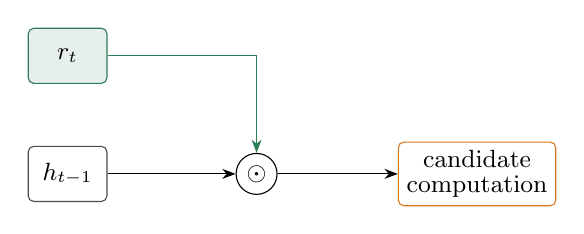
\begin{tikzpicture}
 \node[nbox] (h) at (0,0) {$h_{t-1}$};
 \node[gbox] (r) at (0,1.5) {$r_t$};
 \node[mul] (m) at (2.4,0) {$\odot$};
 \node[nbox,draw=orangec,align=center] (c) at (5.2,0) {candidate\\[-2pt]computation};
 \draw[->] (h)--(m); \draw[->,greenc](r.east)-|(m.north); \draw[->](m)--(c);
\end{tikzpicture}
\caption{Redrawn from slide 35: the previous state is masked by the reset gate before entering the candidate computation.}
\end{figure}

Small reset coefficients suppress previous-state contributions to the candidate; the retained-state branch is controlled \emph{separately} by the update gate.

\begin{example}{Slide 36}{resetnum}
$h_{t-1}=(.8,-.4,.6)^\top$, $r_t=(.1,.9,.5)^\top$ give $h^r_{t-1}=(.08,-.36,.30)^\top$. Feature~1 is strongly attenuated before recurrent mixing; feature~2 contributes $90\%$ of its previous value. The original $h_{t-1}$ still supplies the direct retention branch, whose weight is set by the update gate.
\end{example}

\begin{intuition}
The reset gate answers: ``how much of my past should I \emph{look at} while forming a new proposal?'' Setting $r\approx0$ lets the candidate be computed almost from scratch from $x_t$ (useful when a new segment starts), while $r\approx1$ lets the proposal build on the full history. Crucially it does \emph{not} decide how much of the old state survives in the final output --- that is the update gate's job.
\end{intuition}

\subsection{Constructing the reset-modulated candidate \sltag{37}}

\[
\thh_t=\tanh\big(W_{hx}x_t+W_{hh}(r_t\odot h_{t-1})+b_h\big).
\]
The ``reset-before'' convention masks the previous state \emph{before} recurrent mixing; the current input contributes a separate term.

\begin{figure}[H]\centering
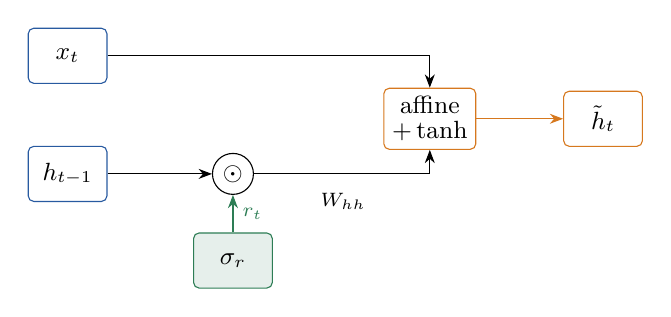
\begin{tikzpicture}
 \node[nbox,draw=bluec] (x) at (0,1.1) {$x_t$};
 \node[nbox,draw=bluec] (h) at (0,-0.4) {$h_{t-1}$};
 \node[gbox] (r) at (2.1,-1.5) {$\sigma_r$};
 \node[mul] (m) at (2.1,-0.4) {$\odot$};
 \node[nbox,draw=orangec,align=center] (a) at (4.6,0.3) {affine\\[-2pt]$+\tanh$};
 \node[nbox,draw=orangec] (c) at (6.8,0.3) {$\thh_t$};
 \draw[->] (h)--(m); \draw[->,greenc] (r.north)--node[right,tick]{$r_t$}(m.south);
 \draw[->] (m.east)-|(a.south); \draw[->] (x.east)-|(a.north); \draw[->,orangec] (a)--(c);
 \node[tick] at (3.5,-0.75) {$W_{hh}$};
\end{tikzpicture}
\caption{Redrawn from slide 37 (reset-before convention). The reset gate itself reads $[x_t;h_{t-1}]$.}
\end{figure}

\subsection{The placement of the reset gate matters \sltag{38}}

\begin{proposition}{Reset-before $\neq$ reset-after}{resetplace}
In general $W(r\odot h)\neq r\odot(Wh)$. Precisely, $W(r\odot h)=(W\diag(r))h$ scales the \emph{columns} of $W$, whereas $r\odot(Wh)=(\diag(r)W)h$ scales its \emph{rows}.
\end{proposition}
\begin{example}{Slide 38}{resetexample}
$W=\begin{pmatrix}1&2\\3&4\end{pmatrix}$, $r=(0.1,0.9)^\top$, $h=(1,1)^\top$. Then $W(r\odot h)=W(0.1,0.9)^\top=(1.9,3.9)^\top$ while $r\odot(Wh)=(0.1,0.9)^\top\odot(3,7)^\top=(0.3,6.3)^\top$.
\end{example}
This lecture and its experiment use \emph{reset-before} recurrent mixing. Other implementations use a \emph{reset-after} affine variant; equations and parameter conventions (e.g.\ separate biases) must be checked before comparing implementations \cite{r10}.

\begin{intuition}
Resetting \emph{before} the matrix means ``hide some \emph{input coordinates} of $h$ from the mixing''; resetting \emph{after} means ``mix everything, then damp some \emph{output coordinates}''. Both look similar in a diagram, but they compute different functions --- so when you copy a GRU from a library, check which one it is.
\end{intuition}

\subsection{The update gate balances retention and replacement \sltag{39--40}}

\begin{definition}{GRU state update}{gruupdate}
\[
z_t=\sigma(W_{zx}x_t+W_{zh}h_{t-1}+b_z),\qquad h_t=z_t\odot h_{t-1}+(1-z_t)\odot\thh_t .
\]
The coefficients $z_t$ and $1-z_t$ are complementary: for every feature the two branch weights sum to one.
\end{definition}

\begin{example}{Slide 39}{gruexample}
$h_{t-1}=(.6,-.4,.2)^\top$, $z_t=(.9,.1,.5)^\top$, $\thh_t=(-.4,.8,-.6)^\top$:
\[
z_t\odot h_{t-1}=(.54,-.04,.10)^\top,\quad(1-z_t)\odot\thh_t=(-.04,.72,-.30)^\top,\quad h_t=(.50,.68,-.20)^\top .
\]
\end{example}

\paragraph{The two gates have different roles (slide 40).}
\begin{center}
\begin{tabular}{llp{4.4cm}}\toprule
Gate & Operation controlled & High coefficient means\\ \midrule
Reset $r_t$ & candidate's historical input & more old context in the candidate\\
Update $z_t$ & final state interpolation & more old state retained\\ \bottomrule
\end{tabular}
\end{center}
For a single component with $h_{t-1}=0.6$ and $\thh_t=-0.4$: $z_t=0.9\Rightarrow h_t=0.54-0.04=0.50$, and $z_t=0.1\Rightarrow h_t=0.06-0.36=-0.30$. Even a nearly closed reset gate can coexist with strong retention of the previous state.

\begin{proposition}{Boundedness of the GRU state}{grubound}
If $|h_{0,j}|\le1$ then $|h_{t,j}|\le1$ for all $t$.
\end{proposition}
\begin{proof}
$|\thh_{t,j}|<1$ and $h_t$ is a convex combination of $h_{t-1}$ and $\thh_t$ (Proposition~\ref{prop:convex}).
\end{proof}

\begin{intuition}
The update gate is a per-coordinate \emph{cross-fader} between ``yesterday's state'' and ``today's proposal''. Unlike the LSTM, where erasing and writing are controlled independently, the GRU ties them: whatever fraction you keep ($z$) is exactly the fraction you give up for the new content ($1-z$). That is why the GRU needs one fewer gate and one fewer state vector.
\end{intuition}

\subsection{Assembling the complete GRU \sltag{41--42}}

\begin{figure}[H]\centering
\resizebox{0.88\linewidth}{!}{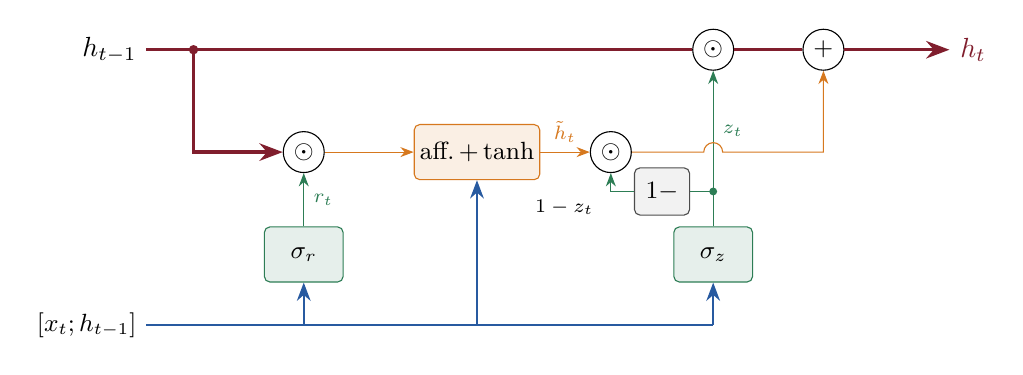
\begin{tikzpicture}
 % bus
 \draw[busp] (-1.0,0.3) -- (6.2,0.3);
 \node[left,font=\small] at (-1.0,0.3) {$[x_t;h_{t-1}]$};
 % top state line
 \node[left] at (-1.0,3.8) {$h_{t-1}$};
 \node[mul] (mz) at (6.2,3.8) {$\odot$};
 \node[mul] (pl) at (7.6,3.8) {$+$};
 \draw[cellp] (-1.0,3.8) -- (mz.west);
 \draw[cellp] (mz.east) -- (pl.west);
 \draw[->,cellp] (pl.east) -- (9.2,3.8) node[right]{$h_t$};
 % reset branch
 \fill[burg] (-0.4,3.8) circle (0.06);
 \node[gbox] (sr) at (1,1.2) {$\sigma_r$};
 \node[mul] (mr) at (1,2.5) {$\odot$};
 \draw[->,cellp] (-0.4,3.8) -- (-0.4,2.5) -- (mr.west);
 \draw[->,busp] (1,0.3) -- (sr.south);
 \draw[->,greenc] (sr.north) -- node[right,tick]{$r_t$} (mr.south);
 % candidate
 \node[cbox,minimum width=15mm] (cd) at (3.2,2.5) {aff.\,+\,$\tanh$};
 \draw[->,orangec] (mr.east) -- (cd.west);
 \draw[->,busp] (3.2,0.3) -- (cd.south);
 \node[mul] (mu) at (4.9,2.5) {$\odot$};
 \draw[->,orangec] (cd.east) -- node[above,tick]{$\tilde h_t$} (mu.west);
 % update gate
 \node[gbox] (sz) at (6.2,1.2) {$\sigma_z$};
 \draw[->,busp] (6.2,0.3) -- (sz.south);
 \draw[greenc] (sz.north) -- (6.2,2.0);
 \draw[->,greenc] (6.2,2.0) -- node[right,tick]{$z_t$} (mz.south);
 \fill[greenc] (6.2,2.0) circle (0.05);
 \node[tbox,minimum width=7mm] (om) at (5.55,2.0) {$1{-}$};
 \draw[greenc] (6.2,2.0) -- (om.east);
 \draw[->,greenc] (om.west) -- (4.9,2.0) -- (mu.south);
 \node[tick,anchor=east] at (4.8,1.8) {$1-z_t$};
 % candidate path with hop over z line
 \draw[->,orangec] (mu.east) -- (6.08,2.5) arc (180:0:0.12) -- (7.6,2.5) -- (pl.south);
\end{tikzpicture}}
\caption{The complete GRU cell, redrawn from slides 41. The reset branch builds a candidate; the update gate controls two final branches with complementary coefficients $z_t$ and $1-z_t$. Each $\sigma$ box includes its own affine map of $[x_t;h_{t-1}]$. (The orange candidate line hops over the green $z_t$ line.)}
\end{figure}

\begin{algorithm}{GRU forward step (slide 42)}{grustep}
\begin{align*}
r_t&=\sigma(W_{rx}x_t+W_{rh}h_{t-1}+b_r),\\
z_t&=\sigma(W_{zx}x_t+W_{zh}h_{t-1}+b_z),\\
\thh_t&=\tanh\big(W_{hx}x_t+W_{hh}(r_t\odot h_{t-1})+b_h\big),\\
h_t&=z_t\odot h_{t-1}+(1-z_t)\odot\thh_t .
\end{align*}
All input matrices are $m\times d$, recurrent matrices $m\times m$, biases $m$. The same parameters are reused across time. An affine prediction readout adds $W_yh_t+b_y$ with output dimension $q$.
\end{algorithm}

% \begin{proposition}{Parameter count of a GRU layer}{gruparams}
% With one bias vector per group, $N_{\rm GRU}=3m(d+m+1)$, plus $q(m+1)$ for the readout. For $d=q=1$, $m=9$: $297+10=307$.
% \end{proposition}
% \begin{proof}
% Three affine groups ($r$, $z$, candidate), each with $md+m^2+m$ scalars.
% \end{proof}

% \subsection{Unfolding a GRU carries one state channel \sltag{43}}

% \begin{figure}[H]\centering
% \begin{tikzpicture}
%  \foreach \k/\l/\xx in {0/{t-1}/0, 1/{t}/4, 2/{t+1}/8}{
%   \node[nbox,minimum width=20mm,minimum height=14mm] (b\k) at (\xx,0) {GRU};
%   \draw[->,busp] (\xx,-1.8) node[below]{$x_{\l}$} -- (b\k.south);
%  }
%  \draw[->,busp] (-2.2,0) node[left]{$h_{t-2}$} -- (b0.west);
%  \draw[->,busp] (b0) -- node[above,tick]{$h_{t-1}$} (b1);
%  \draw[->,busp] (b1) -- node[above,tick]{$h_{t}$} (b2);
%  \draw[->,busp] (b2.east) -- ++(2.2,0) node[right]{$h_{t+1}$};
% \end{tikzpicture}
% \caption{Redrawn from slide 43: one state channel is carried; gates are recomputed at every step from the current input and incoming state; parameters are shared across time.}
% \end{figure}

% \subsection{A GRU also has a direct gradient contribution \sltag{44}}

% Holding the gate and candidate fixed on the direct branch gives
% \[
% \left.\frac{\partial h_t}{\partial h_{t-1}}\right|_{\rm direct}=\diag(z_t).
% \]
% \begin{proposition}{Full GRU Jacobian}{grujac}
% With $J_z=\partial z_t/\partial h_{t-1}$ and $J_{\thh}=\partial\thh_t/\partial h_{t-1}$,
% \[
% J_t=\diag(z_t)+\diag(h_{t-1}-\thh_t)\,J_z+\diag(1-z_t)\,J_{\thh}.
% \]
% Explicitly, $J_z=\diag(z_t\odot(1-z_t))W_{zh}$ and $J_{\thh}=\diag(1-\thh_t^{\,2})\,W_{hh}\big[\diag(r_t)+\diag(h_{t-1}\odot r_t\odot(1-r_t))W_{rh}\big]$ (the second expression is supplementary and uses the reset-before convention; the candidate Jacobian contains the reset-gate dependency).
% \end{proposition}
% \begin{proof}
% Differentiate $h_t=z_t\odot h_{t-1}+(1-z_t)\odot\thh_t$ with the product rule: $\partial(z_t\odot h_{t-1})=\diag(z_t)+\diag(h_{t-1})J_z$, and $\partial((1-z_t)\odot\thh_t)=-\diag(\thh_t)J_z+\diag(1-z_t)J_{\thh}$. Collecting the $J_z$ terms gives $\diag(h_{t-1}-\thh_t)J_z$. For $J_{\thh}$: $\partial(r_t\odot h_{t-1})/\partial h_{t-1}=\diag(r_t)+\diag(h_{t-1})\,\diag(r_t(1-r_t))W_{rh}$ and the outer $\tanh$ contributes $\diag(1-\thh_t^2)W_{hh}$.
% \end{proof}

% \begin{corollary}{Unrolled GRU}{gruunroll}
% Proposition~\ref{prop:directpath} with $g_t=z_t$, $u_t=(1-z_t)\odot\thh_t$ gives
% $h_t=\big(\bigodot_{j=s+1}^{t}z_j\big)\odot h_s+\sum_{k=s+1}^{t}\big(\bigodot_{j=k+1}^{t}z_j\big)\odot(1-z_k)\odot\thh_k .$
% \end{corollary}

% \begin{intuition}
% Same story as the LSTM: a large update gate puts $\diag(z_t)\approx I$ on the direct route, so old information and gradients pass through. The full Jacobian additionally has terms that go through the gates and the candidate (the other two summands), which is why the slide says the complete gradient ``includes all these terms''. Note one difference: in the GRU the retained fraction $z$ and the written fraction $1-z$ are tied, so the \emph{same} gate that protects memory also throttles new writing.
% \end{intuition}

\subsection{Compare the LSTM and GRU mechanisms \sltag{45}}

\begin{center}
\begin{tabular}{lll}\toprule
 & LSTM & GRU\\ \midrule
Recurrent quantities & $(h_t,c_t)$ & $h_t$\\
Gate groups & forget, input, output & reset, update\\
Cell parameters & $4m(d+m+1)$ & $3m(d+m+1)$\\ \bottomrule
\end{tabular}
\end{center}
An output readout adds $q(m+1)$ under the single-bias convention \cite{r11,r7}. Figures~\ref{fig:lstmfull} and the GRU cell figure above are the two diagrams side by side on slide 45.

\begin{intuition}
LSTM $=$ separate eraser, pen and spokesperson, plus a private notebook. GRU $=$ one cross-fader and a context filter, with no separate notebook. The GRU is a leaner design with $25\%$ fewer recurrent parameters at equal width; the LSTM has more independent control. Which one wins is an empirical question \cite{r11}.
\end{intuition}

%=====================================================================
\section{Deep and Bidirectional Gated Recurrent Networks \sltag{46--52}}
%=====================================================================

\subsection{A stacked LSTM has a state pair in every layer \sltag{46}}

\begin{definition}{Stacked LSTM}{stacklstm}
For layers $\ell=1,\dots,L$ and $h^{(0)}_t=x_t$,
\[
\big(h^{(\ell)}_t,c^{(\ell)}_t\big)=\mathrm{LSTM}_{\theta^{(\ell)}}\big(h^{(\ell-1)}_t,\,h^{(\ell)}_{t-1},\,c^{(\ell)}_{t-1}\big).
\]
Hidden outputs pass \emph{upward}; each layer keeps its own cell state and has its own parameters $\theta^{(\ell)}$, shared across time.
\end{definition}

\newcommand{\stackfig}[1]{%
\begin{tikzpicture}
 \foreach \t in {1,2,3}{
  \node[nbox,draw=bluec] (x\t) at (3.4*\t-3.4,0) {$x_\t$};
  \foreach \l in {1,2}{
   \node[nbox,minimum width=16mm,minimum height=9mm] (n\l\t) at (3.4*\t-3.4,1.6*\l) {\ifnum#1=1 LSTM\else GRU\fi$^{(\l)}$};
  }
  \draw[->,busp] (x\t) -- (n1\t);
  \draw[->,busp] (n1\t) -- node[right,tick]{$h^{(1)}_\t$} (n2\t);
  \draw[->,busp] (n2\t.north) -- ++(0,0.5) node[above,tick]{$h^{(2)}_\t$};
 }
 \foreach \l in {1,2}{
  \foreach \a/\b in {1/2,2/3}{
   \ifnum#1=1
    \draw[->,cellp] ($(n\l\a.east)+(0,0.2)$) -- ($(n\l\b.west)+(0,0.2)$);
    \draw[->,busp] ($(n\l\a.east)+(0,-0.2)$) -- ($(n\l\b.west)+(0,-0.2)$);
   \else
    \draw[->,busp] (n\l\a.east) -- (n\l\b.west);
   \fi
  }
 }
 \node[tick,left] at (-1.0,1.6) {layer 1};
 \node[tick,left] at (-1.0,3.2) {layer 2};
\end{tikzpicture}}

\begin{figure}[H]\centering
\stackfig{1}
\caption{Two-layer stacked LSTM unrolled over three steps (redrawn from slide 46). Burgundy: cell states $c^{(\ell)}$; blue: hidden states. $\theta^{(1)}\neq\theta^{(2)}$; each set is shared across the three timesteps.}
\end{figure}

\subsection{A stacked GRU has one state per layer \sltag{47}}

\[
h^{(\ell)}_t=\mathrm{GRU}_{\theta^{(\ell)}}\big(h^{(\ell-1)}_t,\,h^{(\ell)}_{t-1}\big).
\]
\begin{figure}[H]\centering
\stackfig{2}
\caption{Two-layer stacked GRU (redrawn from slide 47): one state per layer, parameters shared across time within each layer.}
\end{figure}

\begin{proposition}{Parameters of stacked gated networks}{stackparams}
With layer widths $m_1,\dots,m_L$ and $m_0=d$,
\[
N_{\rm GRU,stack}=\sum_{\ell=1}^{L}3m_\ell(m_{\ell-1}+m_\ell+1),\qquad N_{\rm readout}=q(m_L+1),
\]
and analogously $\sum_\ell4m_\ell(m_{\ell-1}+m_\ell+1)$ for a stacked LSTM (supplementary).
\end{proposition}
\begin{proof}
Layer $\ell$ receives an input of dimension $m_{\ell-1}$ and has width $m_\ell$, so each affine group has $m_\ell m_{\ell-1}+m_\ell^2+m_\ell$ scalars.
\end{proof}

\begin{intuition}
Stacking adds \emph{depth at every timestep}: layer~1 builds low-level features of the input, layer~2 recurrently processes those features, and so on. Each layer has its own memory timescale. Only the \emph{first} layer sees raw $x_t$; every deeper layer sees the hidden output of the layer below.
\end{intuition}

\subsection{A complete sequence supplies context from both directions \sltag{48}}

For an \emph{offline labelling} task the complete observed sequence is available. Forward processing reads $x_1,\dots,x_T$; backward processing reads the reverse order; the two representations provide different temporal context for the same position \cite{r12}.

\begin{figure}[H]\centering
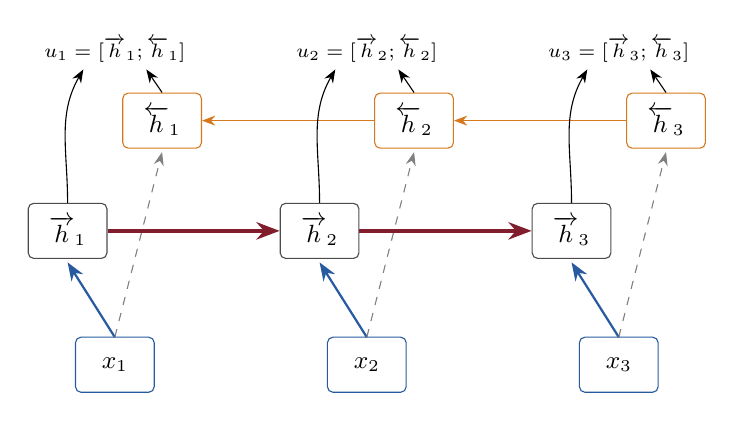
\begin{tikzpicture}
 \foreach \t/\xx in {1/0,2/3.2,3/6.4}{
  \node[nbox,draw=bluec] (x\t) at (\xx,0) {$x_\t$};
  \node[nbox,minimum width=10mm] (f\t) at (\xx-0.6,1.7) {$\overrightarrow{h}_\t$};
  \node[nbox,minimum width=10mm,draw=orangec] (b\t) at (\xx+0.6,3.1) {$\overleftarrow{h}_\t$};
 }
 \foreach \t/\xx in {1/0,2/3.2,3/6.4}{
  \draw[->,busp] (\xx,0.35) -- (\xx-0.6,1.3);
  \draw[->,dashed,gray] (\xx,0.35) -- (\xx+0.6,2.7);
 }
 \draw[->,cellp] (f1)--(f2); \draw[->,cellp](f2)--(f3);
 \draw[->,orangec] (b2)--(b1); \draw[->,orangec](b3)--(b2);
 \foreach \t/\xx in {1/0,2/3.2,3/6.4}{
  \node[tick] at (\xx,4.0) {$u_\t=[\overrightarrow h_\t;\overleftarrow h_\t]$};
  \draw[->,thin] (f\t.north) to[out=90,in=-120] (\xx-0.4,3.75);
  \draw[->,thin] (b\t.north) -- (\xx+0.4,3.75);
 }
\end{tikzpicture}
\caption{Bidirectional context (adapted from slide 48). A forward chain reads left to right, a backward chain right to left; both see every $x_t$ (dashed arrows) and their states are concatenated at each position.}
\end{figure}

\subsection{Forward and backward recurrences use separate parameters \sltag{49}}

\begin{definition}{Bidirectional GRU}{bigru}
\[
\overrightarrow h_t=\mathrm{GRU}_{\theta_\to}(x_t,\overrightarrow h_{t-1}),\quad
\overleftarrow h_t=\mathrm{GRU}_{\theta_\leftarrow}(x_t,\overleftarrow h_{t+1}),\quad
u_t=\begin{bmatrix}\overrightarrow h_t\\ \overleftarrow h_t\end{bmatrix},\quad\hat y_t=\psi(W_yu_t+b_y).
\]
The two directions have independent parameter sets. Boundary states are specified at $t=0$ (forward chain) and $t=T+1$ (backward chain).
\end{definition}

\subsection{A bidirectional LSTM carries four state vectors \sltag{50}}

At every position a bidirectional LSTM produces $(\overrightarrow h_t,\overrightarrow c_t)$ and $(\overleftarrow h_t,\overleftarrow c_t)$:
\[
(\overrightarrow h_t,\overrightarrow c_t)=\mathrm{LSTM}_{\theta_\to}(x_t,\overrightarrow h_{t-1},\overrightarrow c_{t-1}),\qquad
(\overleftarrow h_t,\overleftarrow c_t)=\mathrm{LSTM}_{\theta_\leftarrow}(x_t,\overleftarrow h_{t+1},\overleftarrow c_{t+1}).
\]
Typically the two hidden representations are concatenated for the readout. Each direction maintains its own cell state and gates \cite{r8}. Higher bidirectional layers can receive the concatenated lower-layer hidden outputs.

% \subsection{Bidirectionality must respect information availability \sltag{51}}

% \begin{center}
% \begin{tabular}{p{0.46\linewidth}p{0.46\linewidth}}\toprule
% \textbf{Offline sequence labelling} & \textbf{Online causal prediction}\\ \midrule
% A complete recording can use \emph{later} observed frames to label an earlier position. & At origin $t$, forecasting $x_{t+1}$ can use only information available through $t$.\\ \bottomrule
% \end{tabular}
% \end{center}
% A bidirectional encoder may process a fully observed \emph{history window} for endpoint forecasting; but as new observations arrive its backward representations may need recomputation. Every experiment must match its information access to the intended deployment task \cite{r1}.

% \begin{intuition}
% A bidirectional network is allowed to ``read the whole sentence before deciding what the third word means'' --- legitimate when the sentence is already on the table (tagging a recorded sequence), but \emph{cheating} if the task is predicting the future online. The backward chain at position $t$ depends on $x_T$; in a live system $x_T$ does not exist yet.
% \end{intuition}

% \subsection{Track dimensions and computational costs \sltag{52}}

% With equal directional widths $m$: $u_t\in\R^{2m}$, $W_y\in\R^{q\times2m}$, $b_y\in\R^q$.

% \begin{proposition}{Parameters of bidirectional layers}{biparams}
% $N_{\rm BiLSTM}=8m(d+m+1)$, $N_{\rm BiGRU}=6m(d+m+1)$, plus $q(2m+1)$ for the readout.
% \end{proposition}
% \begin{proof}
% A bidirectional layer contains two independently parameterised cells; each LSTM cell has $4m(d+m+1)$ and each GRU cell $3m(d+m+1)$ parameters. The readout sees $2m$ inputs: $q\cdot2m+q$.
% \end{proof}
% If directional widths differ, the concatenated width is $m_\to+m_\leftarrow$. A second bidirectional layer receiving $u_t$ has input dimension $2m$ rather than $d$ (supplementary: replace $d$ by $2m$ in the formula for that layer).

% \begin{remarkbox}[Depth versus direction]
% Stacking increases depth; bidirectionality adds a second processing direction. Each direction still has \emph{sequential} dependencies (step $t$ needs step $t-1$), and training stores or reconstructs the intermediate information needed for backpropagation through time \cite{r1}. Neither stacking nor bidirectionality removes the sequential bottleneck.
% \end{remarkbox}
% %=====================================================================
% \section{Gated Recurrent Networks in Practice \sltag{53--63}}
% %=====================================================================

% \subsection{Reuse the controlled memory task from Part 1 \sltag{53}}

% The target is an exponentially weighted state:
% \[
% x_t\overset{\rm iid}{\sim}\mathcal N(0,1),\qquad s_t=\alpha s_{t-1}+(1-\alpha)x_t,\qquad y_{t+1}=s_t,\qquad s_0=0 .
% \]
% The primary comparison keeps $\alpha=0.97$ and reuses the \emph{exact} Part~1 input sequences: $16$ training, $4$ validation and $16$ held-out test sequences, each with $1{,}280$ positions, the first $256$ of which warm up the recurrent state. The models predict the next target from the current input and their carried state; the teacher recurrence generates the targets and its coefficient is withheld from the model inputs.

% \begin{proposition}{Time scale and unrolled teacher (supplementary derivation)}{timescale}
% (i) The influence of an input $k$ steps back decays as $\alpha^k=e^{-k/\tau}$ with $\tau=-1/\ln\alpha=\dfrac1{1-\alpha}-\dfrac12+O(1-\alpha)$.\\
% (ii) The teacher is a gated interpolation with constant gate $g=\alpha$ and candidate $x_t$; by Proposition~\ref{prop:directpath}, $s_t=\alpha^{t-s}s_s+(1-\alpha)\sum_{k=s+1}^t\alpha^{t-k}x_k$.\\
% (iii) In stationarity $\mathrm{Var}(s_t)=\dfrac{(1-\alpha)^2}{1-\alpha^2}=\dfrac{1-\alpha}{1+\alpha}$.
% \end{proposition}
% \begin{proof}
% (i) $\alpha^k=e^{k\ln\alpha}=e^{-k/\tau}$ defines $\tau$; with $\varepsilon=1-\alpha$, $-\ln(1-\varepsilon)=\varepsilon+\varepsilon^2/2+\dots$ gives $\tau=\varepsilon^{-1}(1+\varepsilon/2+\dots)^{-1}=\varepsilon^{-1}-\tfrac12+O(\varepsilon)$. (ii) is the unrolled formula with $u_k=(1-\alpha)x_k$. (iii) The weights are $(1-\alpha)\alpha^{j}$ and the $x$'s are independent with unit variance: $(1-\alpha)^2\sum_{j\ge0}\alpha^{2j}=(1-\alpha)^2/(1-\alpha^2)$.
% \end{proof}

% \begin{center}
% \begin{tabular}{cccc}\toprule
% $\alpha$ & $\tau=-1/\ln\alpha$ & stationary SD of $s_t$ (approx.) \\ \midrule
% 0.90 & 9.5 & 0.229\\
% 0.97 & 32.8 & 0.123\\
% 0.99 & 99.5 & 0.071\\ \bottomrule
% \end{tabular}
% \end{center}
% The three timescales $9.5$, $32.8$, $99.5$ are exactly the ones used on slide 60. The stationary SDs are computed here (supplementary) and are only approximate for the finite, warm-up-trimmed sequences; the slides normalise by the empirical training-target SD.

% \begin{figure}[H]\centering
% \begin{tikzpicture}
% \begin{axis}[width=0.72\linewidth,height=5.4cm,xlabel={Lag $k$ (steps)},ylabel={influence $\alpha^k$},xmin=0,xmax=150,ymin=0,ymax=1.05,grid=both,grid style={gray!20},legend pos=north east]
%  \addplot[burg,thick,domain=0:150,samples=150]{exp(x*ln(0.9))};\addlegendentry{$\alpha=.90$}
%  \addplot[orangec,thick,domain=0:150,samples=150]{exp(x*ln(0.97))};\addlegendentry{$\alpha=.97$}
%  \addplot[bluec,thick,domain=0:150,samples=150]{exp(x*ln(0.99))};\addlegendentry{$\alpha=.99$}
%  \addplot[black!60,dashed,domain=0:150]{exp(-1)};
%  \node[tick,anchor=south west] at (axis cs:100,0.38) {$1/e$};
% \end{axis}
% \end{tikzpicture}
% \caption{Original figure: how far back the task requires the model to remember. The dashed line is the $1/e$ level reached at lag $\tau$.}
% \end{figure}

% \begin{intuition}
% The task is a \emph{leaky integrator}: ``the target is a running average with a slowly fading memory''. $\tau\approx33$ steps for $\alpha=0.97$ means roughly the last $33$ inputs matter. Notice that the teacher is \emph{exactly} the gated interpolation of Section~1 with a constant gate $\alpha$ and candidate $x_t$ --- so a gated network only needs to learn ``keep $\approx97\%$ of the state, write $\approx3\%$ of the input''. (Supplementary: a GRU can approximate this with $W_{zx}=W_{zh}=0$, $b_z=\ln\frac{\alpha}{1-\alpha}$ and a nearly linear candidate; this is an observation, not a claim from the slides.) A vanilla RNN has to achieve the same near-identity memory through $W_h$ and $\tanh$.
% \end{intuition}

% \subsection{Match the models by approximate parameter budget \sltag{54}}

% \begin{center}
% \begin{tabular}{lccc}\toprule
% Model & Hidden width & Recurrent-cell parameters & With readout\\ \midrule
% Vanilla RNN & 16 & 288 & 305\\
% LSTM & 8 & 320 & 329\\
% GRU & 9 & 297 & 307\\ \bottomrule
% \end{tabular}
% \end{center}
% All models use $d=q=1$, one recurrent layer and a linear scalar readout, with the single-bias convention: $16(1+16+1)=288$, $4\cdot8(1+8+1)=320$, $3\cdot9(1+9+1)=297$, plus $q(m+1)=17,9,10$.

% Widths differ to obtain similar parameter counts, so the architectures still differ in their state dimensions, gate computations and optimisation dynamics. (Counting stored scalars per step: the RNN carries $16$, the LSTM $8+8=16$, the GRU $9$.)

% \begin{intuition}
% A fair race needs equal \emph{budgets}, not equal widths: since gating costs extra matrices, the gated models are made narrower. Even so, the comparison is not perfectly controlled --- what is tested is ``architecture at a similar number of parameters'', not ``mechanism in isolation''.
% \end{intuition}

% \subsection{Select configurations on validation data \sltag{55}}

% \begin{algorithm}{Common training protocol (slide 55)}{protocol}
% \begin{enumerate}[nosep]
%  \item Adam, global-norm gradient clipping at $1$, chunks of $64$ timesteps (truncated BPTT).
%  \item Carry state values between chunks; \emph{detach} the backward history at chunk boundaries.
%  \item Batch all $16$ independent training sequences; reset states at sequence and epoch boundaries.
%  \item Search learning rates $0.001$ and $0.003$ on training seed $0$ using validation loss.
%  \item Reuse the selected rate for seeds $1$ and $2$; select each checkpoint by validation loss.
%  \item Budget: $90$ epochs, patience $15$; target scaling uses training data only.
% \end{enumerate}
% Test sequences are accessed \emph{only after} configuration and checkpoint selection.
% \end{algorithm}
% This new common protocol differs from Part~1's earlier RNN run.

% \begin{intuition}
% The protocol is the experimental hygiene: hyperparameters and checkpoints are chosen on \emph{validation} data, and the test set is touched once. Carrying state across chunks lets the network use context longer than $64$ steps, while detaching stops gradients from flowing across chunk boundaries (truncated BPTT) so memory cost stays bounded.
% \end{intuition}

% \subsection{Why the earlier RNN error differs \sltag{56}}

% The same $16$-unit RNN has $305$ parameters in both experiments; only the training protocol changes.
% \begin{center}
% \begin{tabular}{lcc}\toprule
%  & Part 1 & Part 2\\ \midrule
% Sequence batch size & 4 & 16\\
% Initial recurrent diagonal & search $\{.8,.95\}$ & fixed $.9$\\
% Selected learning rate & .001 & .003\\
% Maximum epochs / patience & 150 / 20 & 90 / 15\\
% Scored chunk updates per epoch & 64 & 16\\
% Test RMSE & $.0086\pm.0015$ & $.0267\pm.0073$\\ \bottomrule
% \end{tabular}
% \end{center}
% Both use $64$-step TBPTT, zero initial states, state carrying and the same train-target scale; the loss, the validation checkpoint rule and the held-out sequences also coincide.

% \begin{intuition}
% The slide is a lesson in honesty: the \emph{same} vanilla RNN scores $0.0086$ in one protocol and $0.0267$ in another --- a threefold difference with no change in architecture. The table reports two measured protocols; the individual effects of batch size, initialisation, learning rate and update count would require further controlled experiments. Conclusions about architectures are therefore always conditional on the training protocol.
% \end{intuition}

% \subsection{Measured errors on the original memory task \sltag{57}}

% For $\alpha=0.97$, held-out test RMSE (mean $\pm$ sample standard deviation across three independent training seeds; every run scores the same $16$ test sequences in original state units):
% \begin{center}
% \begin{tabular}{lcc}\toprule
% Model & Parameters & Test RMSE\\ \midrule
% Vanilla RNN & 305 & $0.0267\pm0.0073$\\
% LSTM & 329 & $0.0066\pm0.0005$\\
% GRU & 307 & $0.0053\pm0.0009$\\ \bottomrule
% \end{tabular}
% \end{center}
% The gated models achieve lower mean error under this measured protocol; the earlier Part~1 protocol gave RNN RMSE $0.0086\pm0.0015$. Optimisation and selection remain part of the measured comparison \cite{r11}.

% \begin{intuition}
% Gating brings the error down by roughly a factor $4$--$5$ relative to the Part~2 RNN number. As a rough yardstick (supplementary, using the approximate stationary SD $0.123$ from Proposition~\ref{prop:timescale}), a predictor outputting $0$ would have RMSE about $0.12$; the GRU's $0.0053$ is about $4\%$ of that, the LSTM's about $5\%$, the RNN's about $22\%$. The GRU--LSTM gap ($0.0053$ vs.\ $0.0066$) is of the same order as the seed-to-seed SDs ($0.0009$, $0.0005$) with only three seeds, so it should not be over-interpreted; the gated-versus-vanilla gap is much larger than the seed spread.
% \end{intuition}

% \subsection{Predictions and residuals on a common segment \sltag{58--59}}

% Slide 58 compares predictions $\hat y_{t+1}$ (dashed) with the target $y_{t+1}=s_t$ (grey) for RNN, LSTM and GRU on the same held-out segment (first test sequence, observation steps $257$--$436$, training seed $0$, $\alpha=.97$). Slide 59 shows the residuals $e_{t+1}=y_{t+1}-\hat y_{t+1}$ over the same positions, with identical temporal and residual scales (about $\pm4\cdot10^{-2}$); positive residuals indicate underprediction, negative ones overprediction. The reported test RMSE aggregates all $16$ held-out sequences, not just this segment.

% \placeholderfig{58}{3.6cm}{Predictions of RNN, LSTM and GRU (dashed) vs.\ target $y_{t+1}=s_t$ (grey), test sequence 1, steps 257--436, seed 0, $\alpha=.97$. Three panels, axes $[-0.4,0.4]$.}
% \placeholderfig{59}{3.6cm}{Prediction residuals $e_{t+1}=y_{t+1}-\hat y_{t+1}$ on the same segment, identical scales ($\pm4\cdot10^{-2}$), three panels: RNN, LSTM, GRU.}

% \begin{intuition}
% These plots are \emph{sanity checks}: the aggregate RMSE hides \emph{where} a model fails. A model that tracks a slowly drifting target but lags during rapid changes will show systematic, correlated residuals; a model that has learned the leaky integration well leaves residuals that look like small noise.
% \end{intuition}

% \subsection{Increasing the effective memory timescale \sltag{60}}

% Earlier-input influence decays as $\alpha^k=e^{-k/\tau}$ with $\tau=-1/\ln\alpha$, attenuating by $1/e$ at lag $\tau$. The measured values $\alpha=.90,.97,.99$ give $\tau=9.5,\,32.8,\,99.5$ steps. Slide 60 plots, for each of these timescales, the RMSE normalised by the training-target SD of each task (bars, with sample SD over three seeds) for RNN, LSTM and GRU.

% \placeholderfig{60}{4.2cm}{Normalised RMSE (RMSE / training-target SD) against memory timescale $\tau\in\{9.5,32.8,99.5\}$ for RNN, LSTM and GRU; bars show sample SD across three seeds.}

% \begin{intuition}
% Making $\alpha$ larger makes the task \emph{harder in two ways}: the required memory is longer, and the signal $s_t$ becomes smoother and smaller in amplitude, so a fixed absolute error is a larger fraction of it --- hence the normalisation by the target SD. This is the experiment that connects the abstract Jacobian argument of Section~1 to measurable performance: the longer the dependency, the more a network without a dedicated retention mechanism should be expected to struggle. (The numeric bar heights are only in the slide image, hence the placeholder.)
% \end{intuition}

% \subsection{Inspecting learned gate activations \sltag{61--62}}

% \paragraph{LSTM (slide 61).} Each pixel is a learned gate coefficient at one timestep and one hidden feature, with a common colour scale $0$--$1$, for the forget $f_{t,j}$, input $i_{t,j}$ and output $o_{t,j}$ gates ($8$ features, steps $257$--$436$, first test sequence, seed 0, $\alpha=.97$). Feature~4 varies most over time in all three gate families: its forget-gate temporal SD is $.129$, compared with $.009$ for feature~3. The patterns describe coefficient dynamics in these learned coordinates.

% \placeholderfig{61}{4.0cm}{Heat maps of learned LSTM gate activations (forget, input, output; features 1--8; steps 257--436); common colour scale from 0 to 1.}

% \paragraph{GRU (slide 62).} The reset gate controls candidate context; the update gate controls previous-state retention under the lecture convention. Update coefficients have feature-wise temporal means from $.635$ to $.854$ on this segment ($9$ features). Reset feature~3 varies more over time than its update coefficient, with SD $.154$ versus $.052$.

% \placeholderfig{62}{4.0cm}{Heat maps of learned GRU gate activations (reset $r_{t,j}$, update $z_{t,j}$; features 1--9; steps 257--436), common colour scale 0 to 1.}

% \begin{intuition}
% The heat maps show that the gates are not constants: they \emph{move} with the input, and different features behave differently --- most coordinates keep their forget/update value high and nearly steady (long memory) while a few, like LSTM feature~4, fluctuate (short, input-dependent memory). Be careful with interpretation: coordinates are learned, so a pattern in ``feature $j$'' has no meaning outside this trained network and seed.
% \end{intuition}

% \subsection{Choosing mechanisms against the task and resources \sltag{63}}

% \begin{center}
% \begin{tabular}{llll}\toprule
%  & Vanilla RNN & LSTM & GRU\\ \midrule
% State vectors & $h$ & $(h,c)$ & $h$\\
% Gate groups & 0 & 3 & 2\\
% Affine groups & 1 & 4 & 3\\
% Temporal route & recurrent map & cell state & state interpolation\\ \bottomrule
% \end{tabular}
% \end{center}
% All three reuse parameters across time and require sequential state computation. Gating adds learned control and extra affine operations; actual speed and activation storage depend on width, sequence length and implementation. Match information availability, parameter budget and training protocol to the application, and use held-out evidence to assess the resulting trade-offs \cite{r11,r7}.

% \begin{intuition}
% There is no universally best cell. The rules of thumb are: if the task needs long, selective memory, gating is a strong default; between LSTM and GRU, the GRU is leaner, the LSTM offers more separate control; and whatever you pick, compare at matched budgets, with a protocol fixed \emph{before} looking at test data.
% \end{intuition}

%=====================================================================
\section{Summary}
%=====================================================================

\subsection*{Comparison of the architectures covered}

\begin{table}[H]\centering\small
\renewcommand{\arraystretch}{1.2}
\begin{tabular}{@{}>{\raggedright\arraybackslash}p{2.9cm}>{\raggedright\arraybackslash}p{3.6cm}>{\raggedright\arraybackslash}p{3.7cm}>{\raggedright\arraybackslash}p{3.7cm}@{}}\toprule
 & \textbf{Vanilla RNN} & \textbf{LSTM} & \textbf{GRU}\\ \midrule
State & $h_t$ & $(h_t,c_t)$ & $h_t$\\
Gates & none & forget $f$, input $i$, output $o$ & reset $r$, update $z$\\
Memory update & $h_t=\phi(W_xx_t+W_hh_{t-1}+b)$ & $c_t=f\odot c_{t-1}+i\odot\tc_t$ & $h_t=z\odot h_{t-1}+(1-z)\odot\thh_t$\\
Direct Jacobian route & $\diag(\phi')W_h$ & $\diag(f_t)$ & $\diag(z_t)$\\
Cell parameters (single bias) & $m(d+m+1)$ & $4m(d+m+1)$ & $3m(d+m+1)$\\
Bidirectional layer & --- & $8m(d+m+1)$ & $6m(d+m+1)$\\
Readout & \multicolumn{3}{c}{$q(m+1)$; bidirectional: $q(2m+1)$}\\ \midrule
Experiment: width / total params & 16 / 305 & 8 / 329 & 9 / 307\\
Test RMSE ($\alpha=0.97$) & $0.0267\pm0.0073$ & $0.0066\pm0.0005$ & $0.0053\pm0.0009$\\ \bottomrule
\end{tabular}
\caption{Side-by-side comparison of the mechanisms and of the measured results (slides 45, 52, 54, 57, 63).}
\end{table}

% \begin{figure}[H]\centering
% \begin{tikzpicture}
% \begin{axis}[ybar,width=0.66\linewidth,height=5.4cm,symbolic x coords={Vanilla RNN,LSTM,GRU},xtick=data,ymin=0,ymax=0.04,
%  ylabel={Test RMSE ($\alpha=0.97$)},scaled y ticks=false,yticklabel style={/pgf/number format/fixed},bar width=22pt,enlarge x limits=0.3,grid=major,grid style={gray!20},
%  nodes near coords,nodes near coords style={font=\scriptsize,anchor=south west,xshift=2pt},every node near coord/.append style={/pgf/number format/fixed,/pgf/number format/precision=4}]
%  \addplot[fill=burg!70,error bars/.cd,y dir=both,y explicit] coordinates{(Vanilla RNN,0.0267) +- (0,0.0073) (LSTM,0.0066) +- (0,0.0005) (GRU,0.0053) +- (0,0.0009)};
% \end{axis}
% \end{tikzpicture}
% \caption{Qualitative comparison from the numbers on slide 57 (mean $\pm$ sample SD over three seeds; similar parameter budgets: 305, 329, 307). Gated models obtain markedly lower error under this protocol.}
% \end{figure}

\subsection*{Key take-aways}
\begin{itemize}
 \item \textbf{Why gating:} products of Jacobians in a vanilla RNN make long-range information hard to keep; a gate is a learned, elementwise soft mask $g\odot v$ that lets the network \emph{retain}, \emph{forget} and \emph{write} selectively.
 \item \textbf{Additive pathways:} the LSTM cell $c_t=f_t\odot c_{t-1}+i_t\odot\tc_t$ and the GRU interpolation $h_t=z_t\odot h_{t-1}+(1-z_t)\odot\thh_t$ give a direct route with derivative $\diag(f_t)$ or $\diag(z_t)$; retention accumulates as $\prod f$ (or $\prod z$) over time. It helps only when gates are favourable --- the full Jacobian has extra terms.
 \item \textbf{LSTM vs GRU:} the LSTM has two states and three gates ($4m(d+m+1)$ parameters) with independent erase/write/expose control; the GRU has one state and two gates ($3m(d+m+1)$), tying retention to replacement via $z_t$ and $1-z_t$. Mind the reset-before/after convention.
 \item \textbf{Depth and direction:} stacking adds per-layer states; bidirectional networks double the parameters and concatenate forward/backward states, but are valid only when the task grants access to the future context (offline labelling), not for online causal prediction.
%  \item \textbf{Evidence:} on the controlled memory task ($\alpha=0.97$, $\tau\approx33$) the gated models reached test RMSE $0.0066$ (LSTM) and $0.0053$ (GRU) against $0.0267$ for the RNN at similar budgets --- yet the same RNN scored $0.0086$ under the Part~1 protocol, so claims must always be tied to the training protocol and selection on held-out data.
\end{itemize}

\begin{thebibliography}{99}\small
\addcontentsline{toc}{section}{References \emph{(slides 64--66)}}
\bibitem{r1} I.~Goodfellow, Y.~Bengio, A.~Courville, \emph{Deep Learning}. MIT Press, 2016.
\bibitem{r2} A.~Zhang, Z.~C.~Lipton, M.~Li, A.~J.~Smola, \emph{Dive into Deep Learning}. Cambridge University Press, 2024.
\bibitem{r3} K.~P.~Murphy, \emph{Probabilistic Machine Learning: An Introduction}. MIT Press, 2022.
\bibitem{r4} C.~M.~Bishop, H.~Bishop, \emph{Deep Learning: Foundations and Concepts}. Springer, 2024.
\bibitem{r5} S.~Hochreiter, J.~Schmidhuber, ``Long short-term memory,'' \emph{Neural Computation} 9(8):1735--1780, 1997.
\bibitem{r6} F.~A.~Gers, J.~Schmidhuber, F.~Cummins, ``Learning to forget: Continual prediction with LSTM,'' \emph{Neural Computation} 12(10):2451--2471, 2000.
\bibitem{r7} K.~Greff et al., ``LSTM: A search space odyssey,'' \emph{IEEE TNNLS} 28(10):2222--2232, 2017.
\bibitem{r8} A.~Graves, \emph{Supervised Sequence Labelling with Recurrent Neural Networks}. Springer, 2012.
\bibitem{r9} K.~Cho et al., ``Learning phrase representations using RNN encoder--decoder for statistical machine translation,'' EMNLP 2014, pp.\ 1724--1734.
\bibitem{r10} PyTorch Contributors, ``GRU: PyTorch documentation,'' version 2.15, 2026 (accessed November 13, 2026).
\bibitem{r11} J.~Chung, C.~Gulcehre, K.~Cho, Y.~Bengio, ``Empirical evaluation of gated recurrent neural networks on sequence modeling,'' arXiv:1412.3555, 2014.
\bibitem{r12} M.~Schuster, K.~K.~Paliwal, ``Bidirectional recurrent neural networks,'' \emph{IEEE Trans.\ Signal Processing} 45(11):2673--2681, 1997.
\end{thebibliography}

\end{document}